\documentclass[12pt, a4paper]{article}

\usepackage[utf8]{inputenc}
\usepackage[T1]{fontenc}
\usepackage{ngerman}
\usepackage{amsmath, amssymb, amsthm}
\usepackage{mathtools}
\usepackage{bm}
\usepackage{graphicx}
\usepackage{xcolor}
\usepackage{booktabs}
\usepackage{array}
\usepackage{longtable}
\usepackage{geometry}
\usepackage{setspace}
\usepackage{parskip}
\usepackage{hyperref}
\usepackage{cleveref}
\usepackage{natbib}
\usepackage{caption}
\usepackage{subcaption}
\usepackage{algorithm}
\usepackage{algpseudocode}
\usepackage{enumitem}
\usepackage{multirow}
\usepackage{float}
\usepackage{microtype}
\setlist[itemize,1]{label=--}

\geometry{margin=2.5cm, headheight=14pt}
\captionsetup{justification=raggedright, singlelinecheck=false}

% ─── Farben ──────────────────────────────────────────────────────────────────
\definecolor{mainblue}{RGB}{25, 70, 140}
\definecolor{accentred}{RGB}{180, 50, 30}

% ─── Theorem-Umgebungen ───────────────────────────────────────────────────────
\newtheorem{theorem}{Theorem}[section]
\newtheorem{lemma}[theorem]{Lemma}
\newtheorem{proposition}[theorem]{Proposition}
\newtheorem{corollary}[theorem]{Korollar}
\theoremstyle{definition}
\newtheorem{definition}[theorem]{Definition}
\newtheorem{example}[theorem]{Beispiel}
\theoremstyle{remark}
\newtheorem{remark}[theorem]{Bemerkung}
\renewcommand{\proofname}{Beweis}

% ─── Hyperref ────────────────────────────────────────────────────────────────
\hypersetup{
  colorlinks=true,
  linkcolor=mainblue,
  citecolor=accentred,
  urlcolor=mainblue,
  pdftitle={Depension: Eine einheitliche Theorie der mathematischen Abhängigkeitsmodellierung},
  pdfauthor={Stephan Epp},
}

% ─── Makros ──────────────────────────────────────────────────────────────────
\newcommand{\R}{\mathbb{R}}
\newcommand{\C}{\mathbb{C}}
\newcommand{\E}{\mathbb{E}}
\newcommand{\Prob}{\mathbb{P}}
\newcommand{\sigmoid}{\sigma}
\newcommand{\vw}{\bm{w}}
\newcommand{\vx}{\bm{x}}
\newcommand{\vy}{\bm{y}}
\newcommand{\vX}{\bm{X}}
\newcommand{\vA}{\bm{A}}
\newcommand{\vB}{\bm{B}}
\newcommand{\vI}{\bm{I}}
\newcommand{\vP}{\bm{P}}
\newcommand{\vS}{\bm{S}}
\newcommand{\vV}{\bm{V}}
\newcommand{\vLambda}{\bm{\Lambda}}
\newcommand{\T}{\top}
\newcommand{\KL}{\mathrm{KL}}
\newcommand{\diag}{\mathrm{diag}}
\newcommand{\tr}{\mathrm{tr}}
\newcommand{\rank}{\mathrm{rank}}
\newcommand{\re}{\mathrm{Re}}
\newcommand{\DP}{\mathrm{DP}}
\newcommand{\DI}{\mathrm{DI}}
\newcommand{\VIF}{\mathrm{VIF}}
\newcommand{\spec}{\operatorname{spec}}

% ─── Titelseite ──────────────────────────────────────────────────────────────
\title{%
  \textbf{Depension}\\
  {\Large Die Theorie der mathematischen Abhängigkeitsmodellierung}}
\author{Stephan Epp}
\date{30.\ März 2026}

% ════════════════════════════════════════════════════════════════════════════
\begin{document}
% ════════════════════════════════════════════════════════════════════════════

\maketitle
\setcounter{tocdepth}{2}
\tableofcontents
\newpage

% ════════════════════════════════════════════════════════════════════════════
\section{Einleitung und Begriffsentwicklung}
\label{sec:einleitung}
% ════════════════════════════════════════════════════════════════════════════

\subsection{Regression}
Die vorliegende Arbeit führt den neuen wissenschaftlichen Begriff \emph{Depension}
(lat.\ \emph{dependere} = abhängen, griech.\ \emph{-ension} = Zustand, Spannung) ein.
Depension bezeichnet die mathematische Disziplin, die alle Formen der
Abhängigkeitsmodellierung unter einem einheitlichen Rahmen zusammenfasst: statische
Abhängigkeit (lineare Regression), stochastische Abhängigkeit (logistische Regression,
Bernoulli-Modell) und temporale Abhängigkeit (lineare dynamische Systeme, Matrixexponential).

Aufbauend auf drei vorangehenden Arbeiten des Autors -- der logistischen Regression
\citep{epp2026logreg}, den Zustandsklassen dynamischer Systeme
\citep{epp2026sysstate} und der asymmetrischen Matrixmultiplikation
\citep{epp2026systemth} -- werden neue mathematische Konzepte entwickelt und formal
bewiesen: (1) die vier \emph{Depensionsklassen} DP-I bis DP-IV als Verallgemeinerung
der Zustandsklassen KS-I bis KS-IV, (2) der \emph{Depensions-Index} (DI) als
einheitliches Gütemaß über alle Modellklassen, (3) die Äquivalenz zwischen der
Konvexitätsbedingung in der logistischen Regression und der DP-I-Eigenschaft im
dynamischen System, (4) der \emph{Regularisierungs-Klassen-Ãœbergang} als Steuerung
des Eigenwertraums, (5) die Informationsgeometrie der Depension mit der
Fisher-Information als Riemannscher Metrik auf der Depensions-Man\-nig\-fal\-tig\-keit
und (6) die strukturelle Verbindung zwischen VIF-Analyse und
Systemmatrix-Multikollinearität.

Die statistische Methode, die unter dem Namen \emph{Regression} bekannt ist, trägt einen
irreführenden Namen. Das Wort stammt vom lateinischen \emph{regressio} (Rückkehr,
Rückschritt). Der Mathematician Francis Galton prägte ihn 1886 für das Phänomen der
Regression zur Mitte -- die empirische Beobachtung, dass überdurchschnittlich große
Eltern tendenziell Kinder mit etwas geringerer Körpergröße haben.
Das eigentliche Ziel der Methode -- das Erkennen und formale Beschreiben von
Abhängigkeitsbeziehungen zwischen Variablen -- spiegelt sich im Begriff
\emph{Regression} nicht wider.

Dies ist kein bloß sprachkosmetisches Problem. Ein Begriffssystem, das das Wesen
einer Methode nicht trifft, behindert das konzeptionelle Denken und verschleiert
Zusammenhänge zu verwandten Disziplinen. So bleibt die tiefe strukturelle Verbindung
zwischen der logistischen Regression und der Theorie dynamischer Systeme in der
Lehre und Forschung weitgehend unbenannt und ungenutzt.

\subsection{Der neue Begriff: Depension}

\paragraph*{Etymologische Herleitung des Begriffs \emph{Depension}.}
Der Begriff \textbf{Depension} setzt sich zusammen aus:
\begin{itemize}
  \item lat.\ \emph{de-} = von ... ab (Trennung, Abstammung, Abhängigkeit)
  \item lat.\ \emph{pendere} = hängen, abhängen
  \item lat.\ \emph{dependere} = abhängen, in Abhängigkeit stehen
  \item Suffix \emph{-ension} (analog zu \emph{Dimension}, \emph{Tension}, \emph{Extension})
    = etwas, das einen abstrakten mathematischen Zustand beschreibt
\end{itemize}
\medskip\noindent
\textbf{Depension} bezeichnet somit den \emph{mathematischen Zustand des Abhängens} --
das formale Beschreiben und Modellieren von Abhängigkeiten, unabhängig davon, ob diese
statisch, stochastisch oder temporal sind.

Der Begriff trifft präziser als Regression das Wesentliche der Methode: Es geht
nicht um einen Rückschritt, sondern um die mathematische Beschreibung, wie eine
Größe $Y$ von Größen $X_1, \ldots, X_d$ \emph{abhängt} -- also um das
strukturelle Verhältnis der Dependenz.

\begin{remark}[Sprachliche Abgrenzung zu Dependenz]
  Das Wort \emph{Dependenz} (lat.\ \emph{dependentia}) ist bereits in der Statistik
  im Gebrauch (z.\,B.\ lineare Dependenz, Dependenzmaß). \emph{Depension} hebt
  sich davon durch den produktiven Suffix \emph{-ension} ab, der -- wie in
  \emph{Dimension} oder \emph{Tension} -- auf einen formalen, mathematisch
  quantifizierbaren \emph{Zustand} verweist, nicht nur auf eine Beziehung.
  Depension ist demnach das Maß oder der Zustand der Abhängigkeit, während
  Dependenz die Tatsache des Abhängens beschreibt.
\end{remark}

\subsection{Drei Säulen der Depension}

Die vorliegende Arbeit stützt sich auf drei bedeutende Vorarbeiten des Autors, die
nun als Säulen des Depension-Frameworks erkennbar werden:

\begin{enumerate}[label=(\Roman*)]
  \item \textbf{Logistische Regression} \citep{epp2026logreg}: Die logistische
    Regression modelliert die stochastische Abhängigkeit einer binären Zielvariable
    von kontinuierlichen Prädiktoren über die Sigmoid-Transformation und die
    Kreuzentropie-Verlustfunktion. Formal: $\Prob(Y=1|\vx) = \sigmoid(\vw^\T\vx + b)$.
    Dies ist \emph{stochastische Depension}.

  \item \textbf{Zustandsklassen dynamischer Systeme} \citep{epp2026sysstate}: Die
    Systemmatrix $\vA$ eines linearen dynamischen Systems $\dot{\vx} = \vA\vx$
    beschreibt, wie der Zustandsvektor $\vx(t)$ von seiner Vergangenheit
    $\vx(0)$ abhängt: $\vx(t) = e^{\vA t}\vx(0)$. Die Zustandsklassen KS-I bis
    KS-IV klassifizieren das Langzeitverhalten dieser Abhängigkeit.
    Dies ist \emph{temporale Depension}.

  \item \textbf{Asymmetrische Matrixstruktur} \citep{epp2026systemth}: Die
    semantische Dualität zwischen Zeilen (Aggregation, Empfänger) und Spalten
    (Ausbreitung, Sender) einer Systemmatrix beschreibt die \emph{Richtungs\-struktur}
    der Abhängigkeit. Dies ist \emph{strukturelle Depension}.
\end{enumerate}

\begin{figure}[H]
  \centering
  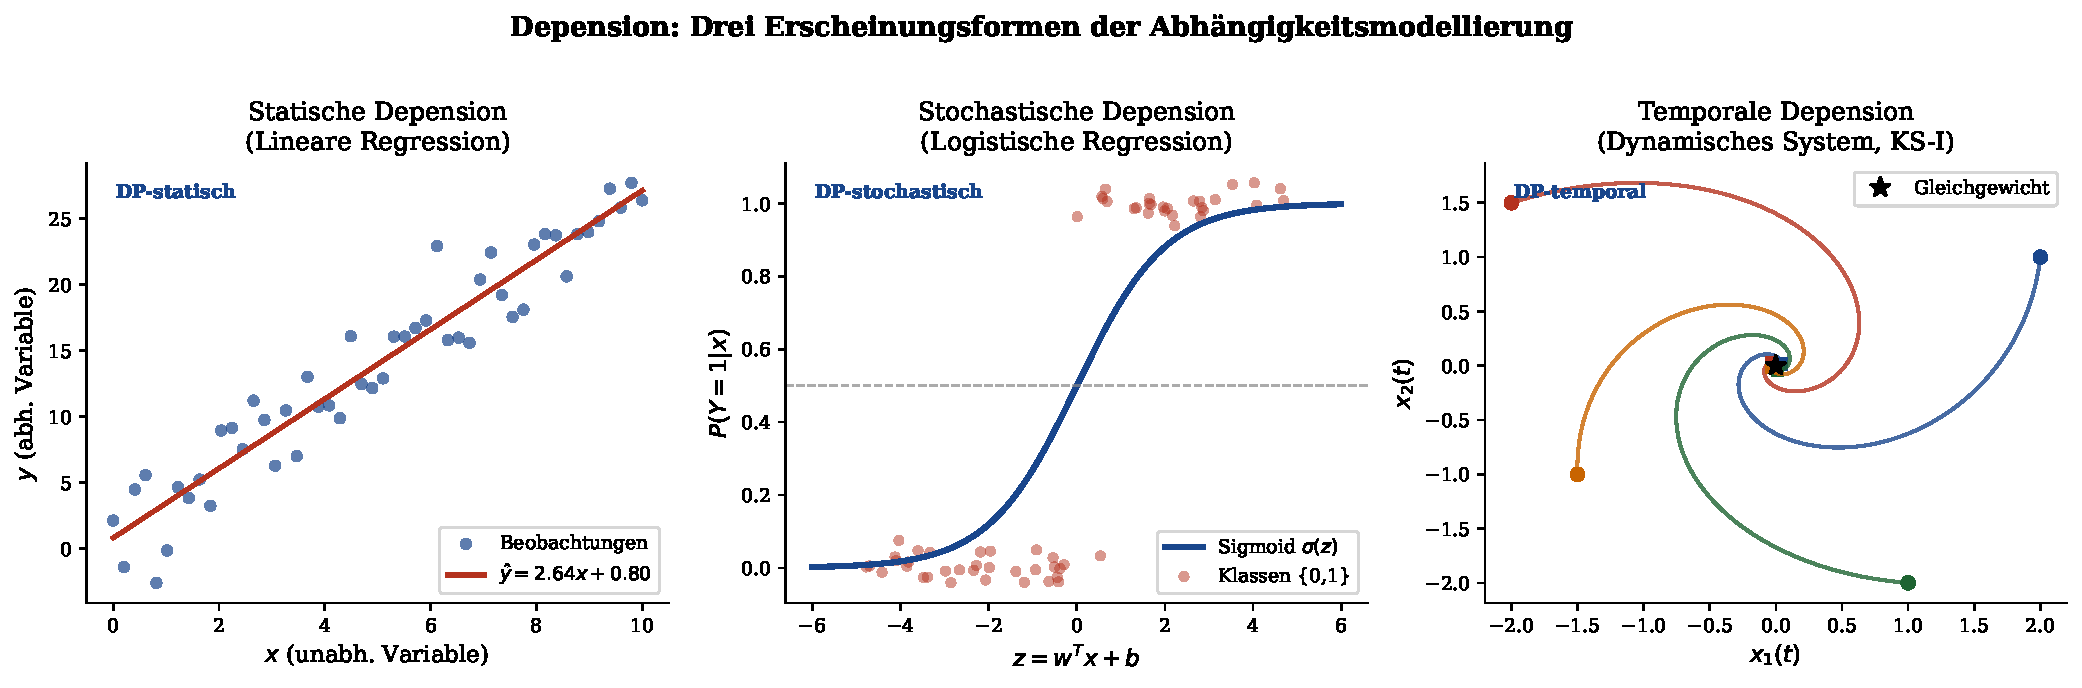
\includegraphics[width=\textwidth]{fig_depension_concept.pdf}
  \caption{Die drei Erscheinungsformen der Depension: Links die statische (lineare
    Regression als Grenzfall), Mitte die stochastische (logistische Regression) und
    rechts die temporale Depension (Trajektorien eines KS-I-Systems). Allen gemeinsam
    ist die fundamentale Frage: Wie hängt $Y$ von $X$ ab?}
  \label{fig:konzept}
\end{figure}

\textbf{Abbildung~\ref{fig:konzept}} stellt die drei Erscheinungsformen der Depension
nebeneinander. Links sehen wir die klassische Regressionsgerade als Modell für eine
lineare statische Abhängigkeit. In der Mitte zeigt die Sigmoid-Kurve, wie die logistische
Regression eine probabilistische Abhängigkeit modelliert -- nicht eine lineare, sondern
eine sigmoidal gebogene. Rechts sehen wir die Trajektorien eines stabilen dynamischen
Systems: Alle Anfangszustände konvergieren zum Ursprung, was zeigt, dass der aktuelle
Zustand $\vx(t)$ vollständig vom Anfangszustand $\vx(0)$ \emph{abhängt} -- dies ist
die reinste Form der temporalen Depension.

\subsection{Aufbau der Arbeit}

Kapitel~\ref{sec:grundlagen} entwickelt die mathematischen Grundlagen der Depension
auf drei Ebenen. Kapitel~\ref{sec:klassen} definiert die Depensionsklassen DP-I bis
DP-IV als Verallgemeinerung der Zustandsklassen. Kapitel~\ref{sec:neue_aussagen}
enthält die zentralen neuen Theoreme und Beweise -- insbesondere den Zusammenhang
zwischen Konvexität in der Regression und DP-I-Eigenschaft in der Systemtheorie,
den Depensions-Index sowie das Regularisierungs-Klassen-Ãœbergangstheorem.
Kapitel~\ref{sec:infogeom} behandelt die Informationsgeometrie der Depension.
Kapitel~\ref{sec:sparse} verbindet VIF-Analyse und strukturelle Depension.
Kapitel~\ref{sec:experimente} präsentiert und interpretiert alle numerischen
Experimente. Kapitel~\ref{sec:ausblick} gibt einen Ausblick.

% ════════════════════════════════════════════════════════════════════════════
\section{Mathematische Grundlagen der Depension}
\label{sec:grundlagen}
% ════════════════════════════════════════════════════════════════════════════

\subsection{Definition des Depensions-Operators}

\begin{definition}[Depensions-Operator]
\label{def:depop}
Sei $\mathcal{X}$ ein Eingaberaum und $\mathcal{Y}$ ein Ausgaberaum. Ein
\emph{Depensions-Operator} ist eine messbare Abbildung
\begin{equation}
  \mathcal{D} : \mathcal{X} \to \mathcal{P}(\mathcal{Y}),
  \label{eq:depop}
\end{equation}
die jedem Eingabewert $x \in \mathcal{X}$ eine Wahrscheinlichkeitsverteilung über
$\mathcal{Y}$ zuordnet. Der Wert $\mathcal{D}(x)$ heißt die
\emph{bedingte Depension} von $Y$ gegeben $x$.
\end{definition}

\begin{remark}
Für deterministische Ausgaben degeneriert $\mathcal{D}(x)$ zu einem Dirac-Maß
$\delta_{f(x)}$, und die Depension reduziert sich auf eine gewöhnliche Funktion
$f: \mathcal{X} \to \mathcal{Y}$.
\end{remark}

Die klassischen Modelle sind nun Spezialfälle:

\begin{example}[Statische Depension: Lineare Regression]
  Für $\mathcal{X} = \R^d$, $\mathcal{Y} = \R$ und $Y|\vx \sim \mathcal{N}(\vw^\T\vx + b,\,\sigma^2)$:
  \[
    \mathcal{D}_{\rm lin}(\vx) = \mathcal{N}(\vw^\T\vx + b,\,\sigma^2).
  \]
  Der lineare Prädiktor $\vw^\T\vx + b$ ist der \emph{lokale Depensions-Parameter}.
\end{example}

\begin{example}[Stochastische Depension: Logistische Regression]
\label{ex:logdep}
  Für $\mathcal{X} = \R^d$, $\mathcal{Y} = \{0,1\}$:
  \[
    \mathcal{D}_{\rm log}(\vx) = \mathrm{Bern}\!\bigl(\sigmoid(\vw^\T\vx + b)\bigr),
  \]
  wobei $\sigmoid(z) = (1+e^{-z})^{-1}$ die Sigmoid-Funktion ist. Die Abhängigkeit
  von $\vx$ wird durch das Odds-Verhältnis $e^{\vw^\T\vx+b}$ quantifiziert.
\end{example}

\begin{example}[Temporale Depension: Dynamisches System]
\label{ex:tempdep}
  Für das LTI-System $\dot{\vx}(t) = \vA\vx(t)$ mit $\vx(0) = \vx_0$:
  \[
    \mathcal{D}_{\rm dyn}(\vx_0, t) = \delta_{e^{\vA t}\vx_0}.
  \]
  Die Abhängigkeit des Zustands $\vx(t)$ vom Anfangszustand $\vx_0$ wird durch den
  \emph{Übergangsoperator} $e^{\vA t}$ vollständig beschrieben.
\end{example}

\subsection{Grundlegende algebraische Struktur}

Allen drei Depensionsformen liegt dieselbe algebraische Kernstruktur zugrunde:

\begin{proposition}[Gemeinsame algebraische Struktur der Depension]
\label{prop:struktur}
Die drei kanonischen Depensionsformen besitzen eine gemeinsame Struktur, die sich
in einer zentralen Matrix und einem linearen Prädiktor manifestiert:

\begin{center}
\renewcommand{\arraystretch}{1.6}
\begin{tabular}{llll}
\toprule
Form & Zentrale Matrix & Linearer Prädiktor & Outputfunktion \\
\midrule
Statisch (lin.) & $\vX^\T\vX$ & $\vw^\T\vx$ & $f(z) = z$ \\
Stochastisch (log.) & $\vX^\T\vS\vX$ & $\vw^\T\vx + b$ & $f(z) = \sigmoid(z)$ \\
Temporal (dyn.) & $e^{\vA t}$ & $\vA\vx$ & $f(t,\vx_0) = e^{\vA t}\vx_0$ \\
\bottomrule
\end{tabular}
\end{center}
Die Konvexitäts-/Stabilitätseigenschaft ist in allen drei Fällen durch die
Eigenwerte der zentralen Matrix bestimmt.
\end{proposition}

\begin{proof}
Für die lineare Regression ist die quadratische Verlustfunktion konvex genau dann,
wenn $\vX^\T\vX \succeq 0$, was stets gilt. Für die logistische Regression gilt
$\nabla^2\mathcal{L} = \frac{1}{n}\vX^\T\vS\vX \succeq 0$ (Theorem~\ref{thm:konvex_aequiv}
unten). Für das dynamische System ist der Übergangsoperator $e^{\vA t}$ genau dann
beschränkt für alle $t \geq 0$, wenn alle Eigenwerte von $\vA$ nicht-positiven Realteil
haben (Zustandsklasse KS-I/II). Die Verbindung ist nicht zufällig: In allen Fällen
bestimmt das Spektrum einer zentralen Matrix das Langzeitverhalten.
\end{proof}

\subsection{Die Sigmoid-Funktion als Depensions-Verbindungsglied}

\begin{proposition}[Sigmoid als stochastischer Depensions-Operator]
\label{prop:sigmoid}
Die Sigmoid-Funktion $\sigmoid: \R \to (0,1)$ ist das kanonische Verbindungsglied
zwischen dem linearen Prädiktor und der stochastischen Depension. Sie besitzt
folgende Eigenschaften, die sie für diesen Zweck qualifizieren:
\begin{enumerate}[label=(\roman*)]
  \item $\sigmoid$ ist streng monoton wachsend und glatt ($\sigmoid \in C^\infty$).
  \item Die Ableitung $\sigmoid'(z) = \sigmoid(z)(1-\sigmoid(z)) \in (0, 1/4]$
    ist die Fisher-Information der Bernoulli-Depension am Arbeitspunkt $z$.
  \item Die Log-Odds-Linearität $\ln\frac{\sigmoid(z)}{1-\sigmoid(z)} = z$ garantiert
    die interpretierbare Parametrisierung über Odds-Ratios.
  \item Als Verteilungsfunktion der logistischen Verteilung ist $\sigmoid$ die
    kanonische Link-Funktion des Bernoulli-GLM.
\end{enumerate}
\end{proposition}

% ════════════════════════════════════════════════════════════════════════════
\section{Depensionsklassen DP-I bis DP-IV}
\label{sec:klassen}
% ════════════════════════════════════════════════════════════════════════════

Die Zustandsklassen KS-I bis KS-IV aus \citet{epp2026sysstate} klassifizieren das
Langzeitverhalten linearer dynamischer Systeme anhand der Spektralabszisse ihrer
Systemmatrix. Das Depensions-Framework verallgemeinert diese Klassifikation auf
beliebige Depensionsmodelle.

\subsection{Definition der Depensionsklassen}

\begin{definition}[Depensionsklassen DP-I bis DP-IV]
\label{def:dpklassen}
Sei $\mathcal{M}$ ein Depensionsmodell mit zentraler Matrix $\mathbf{M}$ und
sei $\spec(\mathbf{M}) = \{\lambda_1, \ldots, \lambda_n\} \subset \C$ das Spektrum.
Die \emph{Depensionsklasse} $\DP(\mathcal{M})$ ist definiert durch:
\begin{align}
  \DP\text{-I}  &: \quad \max_k \re(\lambda_k) < 0
    \quad\text{(konvergente Depension)}
    \label{eq:dp1} \\
  \DP\text{-II} &: \quad \max_k \re(\lambda_k) \leq 0 \;\wedge\;
    \exists\,k:\,\re(\lambda_k) = 0 \text{ (semieinfach)}
    \quad\text{(grenzstabile Depension)}
    \label{eq:dp2} \\
  \DP\text{-III}&: \quad \max_k \re(\lambda_k) > 0 \;\wedge\;
    \min_k \re(\lambda_k) \geq 0
    \quad\text{(divergente Depension)}
    \label{eq:dp3} \\
  \DP\text{-IV} &: \quad \max_k \re(\lambda_k) > 0 \;\wedge\;
    \min_k \re(\lambda_k) < 0
    \quad\text{(hyperbolische Depension)}
    \label{eq:dp4}
\end{align}
\end{definition}

\begin{figure}[H]
  \centering
  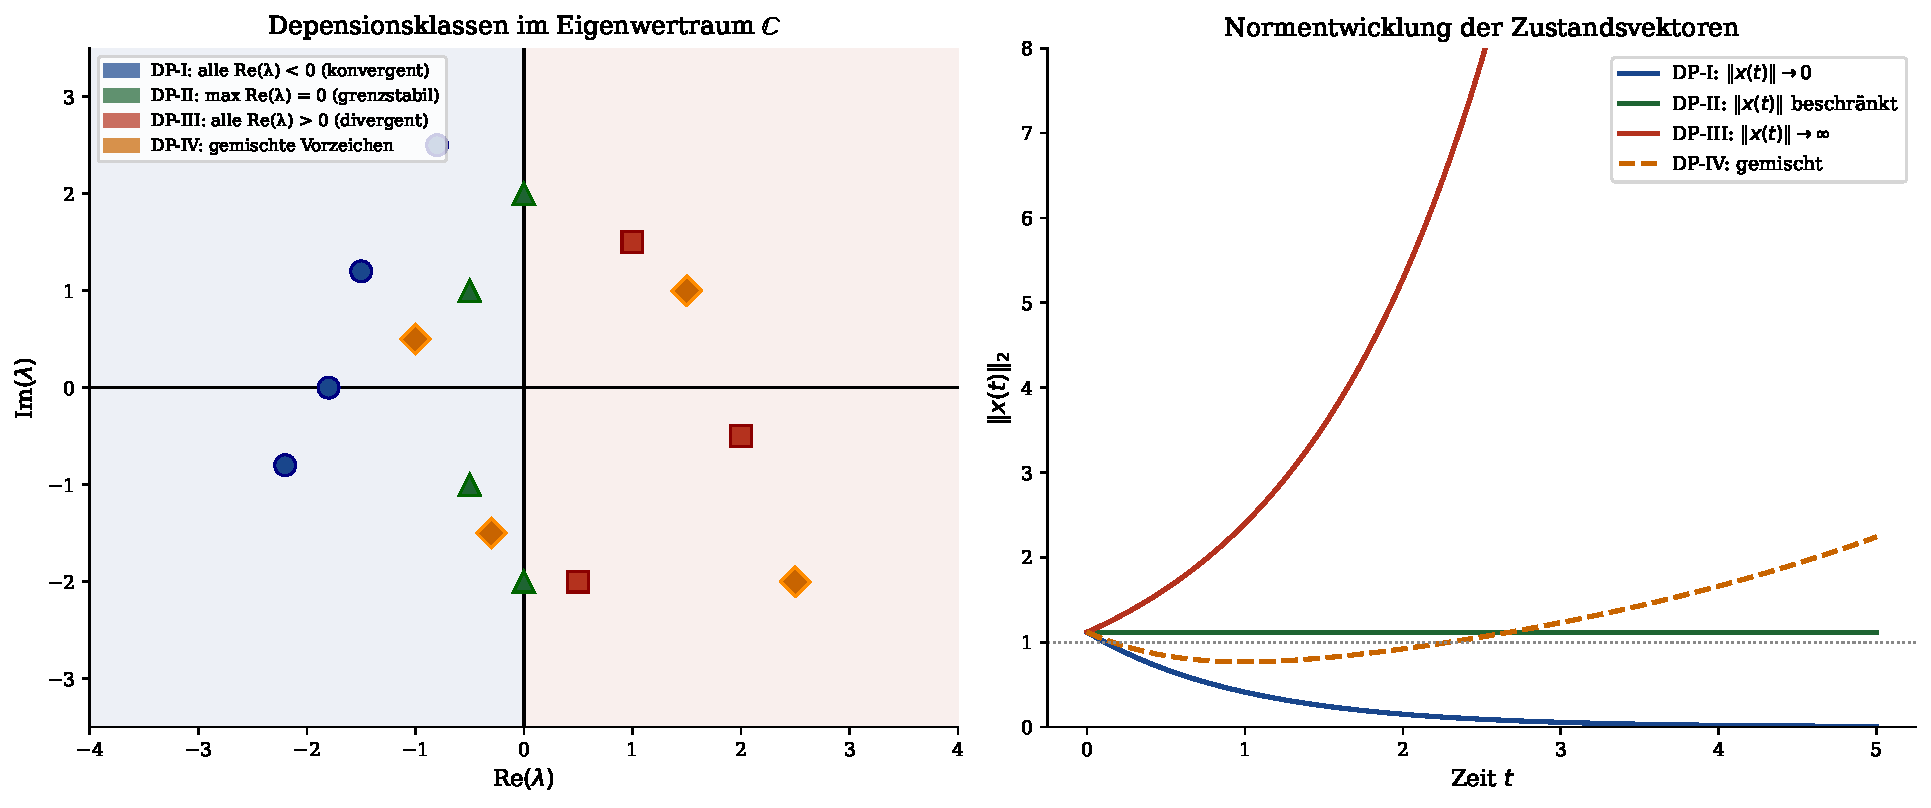
\includegraphics[width=\textwidth]{fig_depension_klassen.pdf}
  \caption{Links: Lage der Eigenwerte im komplexen Eigenwertraum $\C$ für
    die vier Depensionsklassen DP-I (blau, alle $\re(\lambda)<0$),
    DP-II (grün, $\max\re(\lambda)=0$), DP-III (rot, alle $\re(\lambda)>0$)
    und DP-IV (orange, gemischte Vorzeichen). Rechts: Zeitliche Entwicklung
    der Norm $\|x(t)\|_2$ für alle vier Klassen. DP-I konvergiert exponentiell,
    DP-II bleibt beschränkt (Oszillation), DP-III divergiert, DP-IV zeigt
    gemischtes Verhalten.}
  \label{fig:klassen}
\end{figure}

\textbf{Abbildung~\ref{fig:klassen}} zeigt die Klassifikation im Eigenwertraum und
die daraus resultierenden Zeitverläufe auf eine besonders anschauliche Weise. Im
linken Teilbild sind vier Gruppen von Eigenwerten eingetragen: Die blauen Kreise
(DP-I) liegen vollständig links der imaginären Achse -- jede Komponente des
Zustandsvektors klingt exponentiell ab. Die grünen Dreiecke (DP-II) liegen auf oder
links der Achse, mit mindestens einem auf der Achse -- persistente Oszillationen ohne
Wachstum. Die roten Quadrate (DP-III) liegen alle rechts der Achse -- jede Komponente
wächst exponentiell. Die orangen Rauten (DP-IV) haben Eigenwerte beidseits der Achse
-- ein Sattelpunkt mit stablerem und instabilem Unterraum.

Das rechte Teilbild bestätigt diese Analyse durch die Normentwicklung
$\|x(t)\|_2$: DP-I (blau) fällt monoton gegen null, DP-II (grün) bleibt konstant
auf einem Niveau, DP-III (rot) explodiert exponentiell, und DP-IV (orange, gestrichelt)
zeigt ein komplexes Verhalten, das von der Anfangsbedingung abhängt.

\subsection{Eigenschaften der Depensionsklassen}

\begin{theorem}[Endlichkeit der Depension nach Klasse]
\label{thm:endlichkeit_dp}
Für ein Depensionsmodell mit zentraler Matrix $\mathbf{M}$ gilt:
\begin{enumerate}[label=(\roman*)]
  \item $\DP(\mathcal{M}) = \DP\text{-I}$ $\Rightarrow$ Der Depensions-Operator
    $e^{\mathbf{M}t}$ ist für alle $t \geq 0$ beschränkt, und
    $\|e^{\mathbf{M}t}\| \to 0$.
  \item $\DP(\mathcal{M}) = \DP\text{-II}$ $\Rightarrow$
    $\sup_{t \geq 0}\|e^{\mathbf{M}t}\| < \infty$ (Endlichkeit), aber
    kein Abklingen.
  \item $\DP(\mathcal{M}) \in \{\DP\text{-III}, \DP\text{-IV}\}$ $\Rightarrow$
    $\|e^{\mathbf{M}t}\| \to \infty$ für generische Anfangsbedingungen
    (keine Endlichkeit).
\end{enumerate}
\end{theorem}

\begin{proof}
Die Aussagen (i) und (ii) folgen aus Theorem~3.1 und Theorem~3.2 in
\citet{epp2026sysstate} (Eigenschaften KS-I und KS-II), da die Depensionsklassen
DP-I und DP-II direkt den Zustandsklassen KS-I und KS-II entsprechen. Für (iii):
Sei $\vA = \mathbf{M}$ und $\lambda^* = \alpha^* + i\beta^*$ ein Eigenwert mit
$\re(\lambda^*) = \alpha^* > 0$. Mit dem zugehörigen Eigenvektor $\bm{v}^*$ gilt:
\[
  \|e^{\mathbf{M}t}\vx_0\| \geq |\langle\bm{v}^*, e^{\mathbf{M}t}\vx_0\rangle|
  = e^{\alpha^* t} |\langle\bm{v}^*, \vx_0\rangle| \cdot |\cos(\beta^* t + \phi)|.
\]
Für generische $\vx_0$ (d.\,h.\ $\langle\bm{v}^*, \vx_0\rangle \neq 0$) wächst
dies unbeschränkt. \qedhere
\end{proof}

\begin{figure}[H]
  \centering
  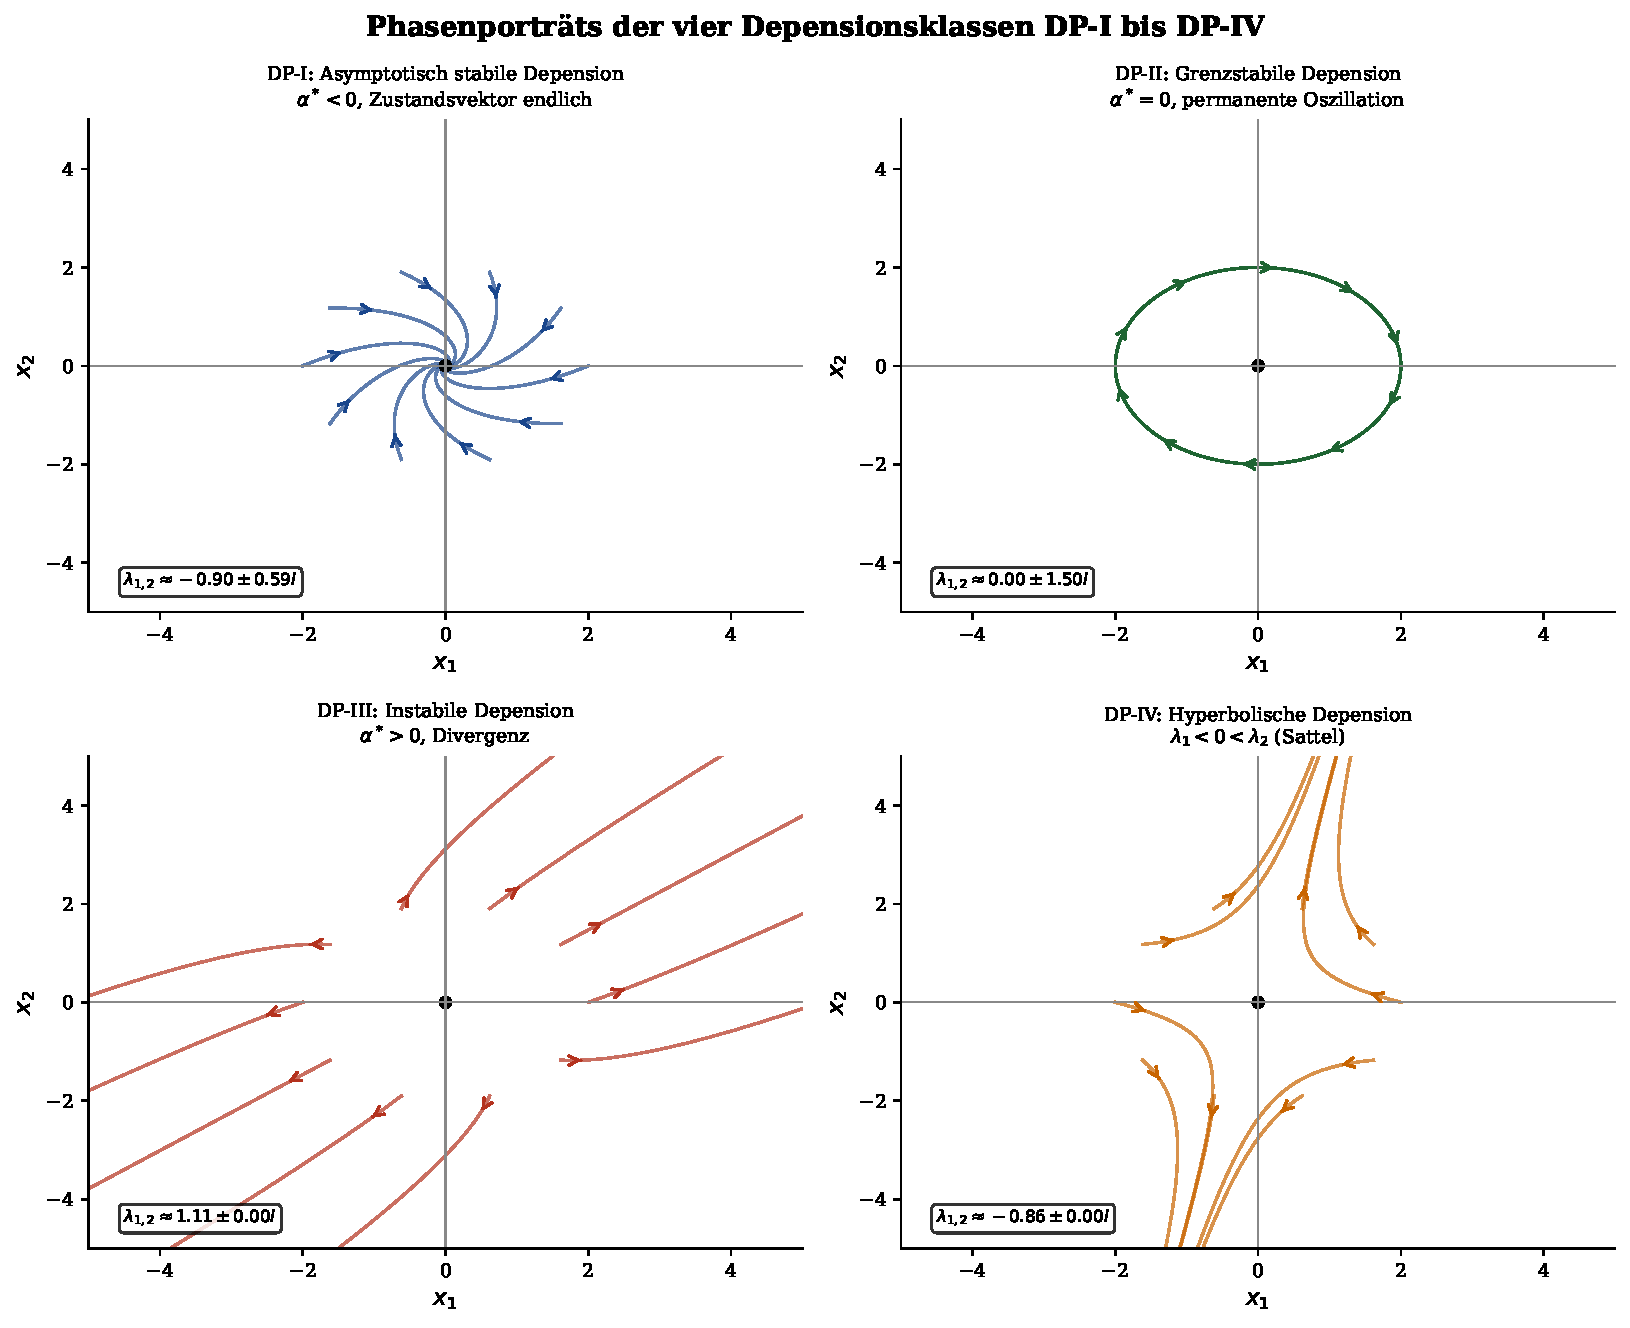
\includegraphics[width=\textwidth]{fig_phasenportrait_klassen.pdf}
  \caption{Phasenporträts der vier Depensionsklassen für ein 2D-System.
    DP-I (oben links): Alle Trajektorien konvergieren stabil zum Ursprung --
    die Depension ist vollständig durch den Anfangszustand bestimmt und klingt ab.
    DP-II (oben rechts): Elliptische Orbits -- persistente Zeitabhängigkeit ohne
    Wachstum oder Abklingen; die Depension bleibt konstant in ihrer Stärke.
    DP-III (unten links): Alle Trajektorien entfernen sich vom Ursprung -- die
    Depension wächst, Vorhersagen werden zunehmend unzuverlässig.
    DP-IV (unten rechts): Sattelpunkt -- stabile und instabile Mannigfaltigkeit
    kreuzen sich; nur Anfangsbedingungen auf der stabilen Mannigfaltigkeit zeigen
    Konvergenz.}
  \label{fig:phasen}
\end{figure}

Die Phasenporträts in Abbildung~\ref{fig:phasen} illustrieren den qualitativen
Unterschied zwischen den Klassen auf unmittelbar anschauliche Weise. Für ein
2D-System zeigt DP-I einen stabilen Knoten oder Fokus -- unabhängig vom
Startpunkt konvergiert jede Bahn zum Ursprung. DP-II offenbart konzentrische
Ellipsen: Die Depension bleibt konstant stark, ändert aber ständig ihre Richtung.
DP-III zeigt einen instabilen Knoten -- jede Störung wächst exponentiell an. DP-IV
schließlich zeigt die charakteristische Sattelstruktur mit genau einer stabilen und
einer instabilen Richtung.

% ════════════════════════════════════════════════════════════════════════════
\section{Neue mathematische Aussagen und Beweise}
\label{sec:neue_aussagen}
% ════════════════════════════════════════════════════════════════════════════

\subsection{Äquivalenz: Konvexität als DP-I-Eigenschaft}

Das zentrale Verbindungstheorem zwischen der logistischen Regression und der
Systeme-Theorie lautet:

\begin{theorem}[Äquivalenz von Konvexität und DP-I-Eigenschaft]
\label{thm:konvex_aequiv}
\textup{(Neu)} Sei $\mathcal{L}(\vw)$ die binäre Kreuzentropie-Verlustfunktion
der logistischen Regression und $H(\vw) = \nabla^2\mathcal{L}(\vw)$ die Hesse-Matrix.
Die folgenden Aussagen sind äquivalent:
\begin{enumerate}[label=(\roman*)]
  \item Die Verlustfunktion $\mathcal{L}$ ist strikt konvex.
  \item Alle Eigenwerte von $H$ sind strikt positiv: $\spec(H) \subset (0, \infty)$.
  \item Das Gradientenfluss-System
    $\dot{\vw}(t) = -\nabla\mathcal{L}(\vw(t))$
    linearisiert um $\vw^*$ besitzt die Depensionsklasse DP-I.
  \item Der Gradient-Abstieg konvergiert linear mit Rate $1 - \eta\mu$, wobei
    $\mu = \lambda_{\min}(H) > 0$.
\end{enumerate}
\end{theorem}

\begin{proof}
  \textbf{(i) $\Leftrightarrow$ (ii):} Die Funktion $\mathcal{L}$ ist strikt konvex
  genau dann, wenn $H(\vw) \succ 0$ für alle $\vw$, d.\,h.\ alle Eigenwerte von
  $H$ sind strikt positiv \citep[Theorem~4.1]{epp2026logreg}.

  \textbf{(ii) $\Rightarrow$ (iii):} Das Gradientenfluss-System lautet in
  linearisierter Form um das Minimum $\vw^*$:
  \[
    \dot{\delta\vw}(t) = -H(\vw^*)\, \delta\vw(t),
  \]
  wobei $\delta\vw(t) = \vw(t) - \vw^*$. Die Systemmatrix ist $\vA = -H(\vw^*)$.
  Da $\spec(H(\vw^*)) \subset (0,\infty)$, gilt $\spec(\vA) = \spec(-H) \subset (-\infty, 0)$.
  Damit ist $\max_k\re(\lambda_k(\vA)) < 0$ -- die Definition von DP-I.

  \textbf{(iii) $\Rightarrow$ (iv):} Aus DP-I folgt $\|e^{\vA t}\| \leq c\,e^{-\mu t}$
  mit $\mu = \lambda_{\min}(H) > 0$. Der diskrete Gradientenabstieg $\vw^{(k+1)} =
  \vw^{(k)} - \eta\nabla\mathcal{L}(\vw^{(k)})$ approximiert den Gradientenfluss,
  und die lineare Konvergenzrate folgt aus der starken Konvexität.

  \textbf{(iv) $\Rightarrow$ (i):} Lineare Konvergenz setzt voraus, dass die
  Verlustfunktion stark konvex ist, was strikte Konvexität impliziert. \qedhere
\end{proof}

\begin{corollary}[Gradientenabstieg als DP-I-System]
\label{cor:gd_dp1}
\textup{(Neu)} Der Gradientenabstieg für die logistische Regression \emph{ist} ein
dynamisches System der Klasse DP-I. Die Eigenwerte der Systemmatrix $\vA = -H(\vw^*)$
entsprechen den negativierten Eigenwerten der Hesse-Matrix; die Konvergenzrate des
Optimierungsverfahrens ist identisch mit der Abklingrate des dynamischen Systems.
\end{corollary}

\begin{figure}[H]
  \centering
  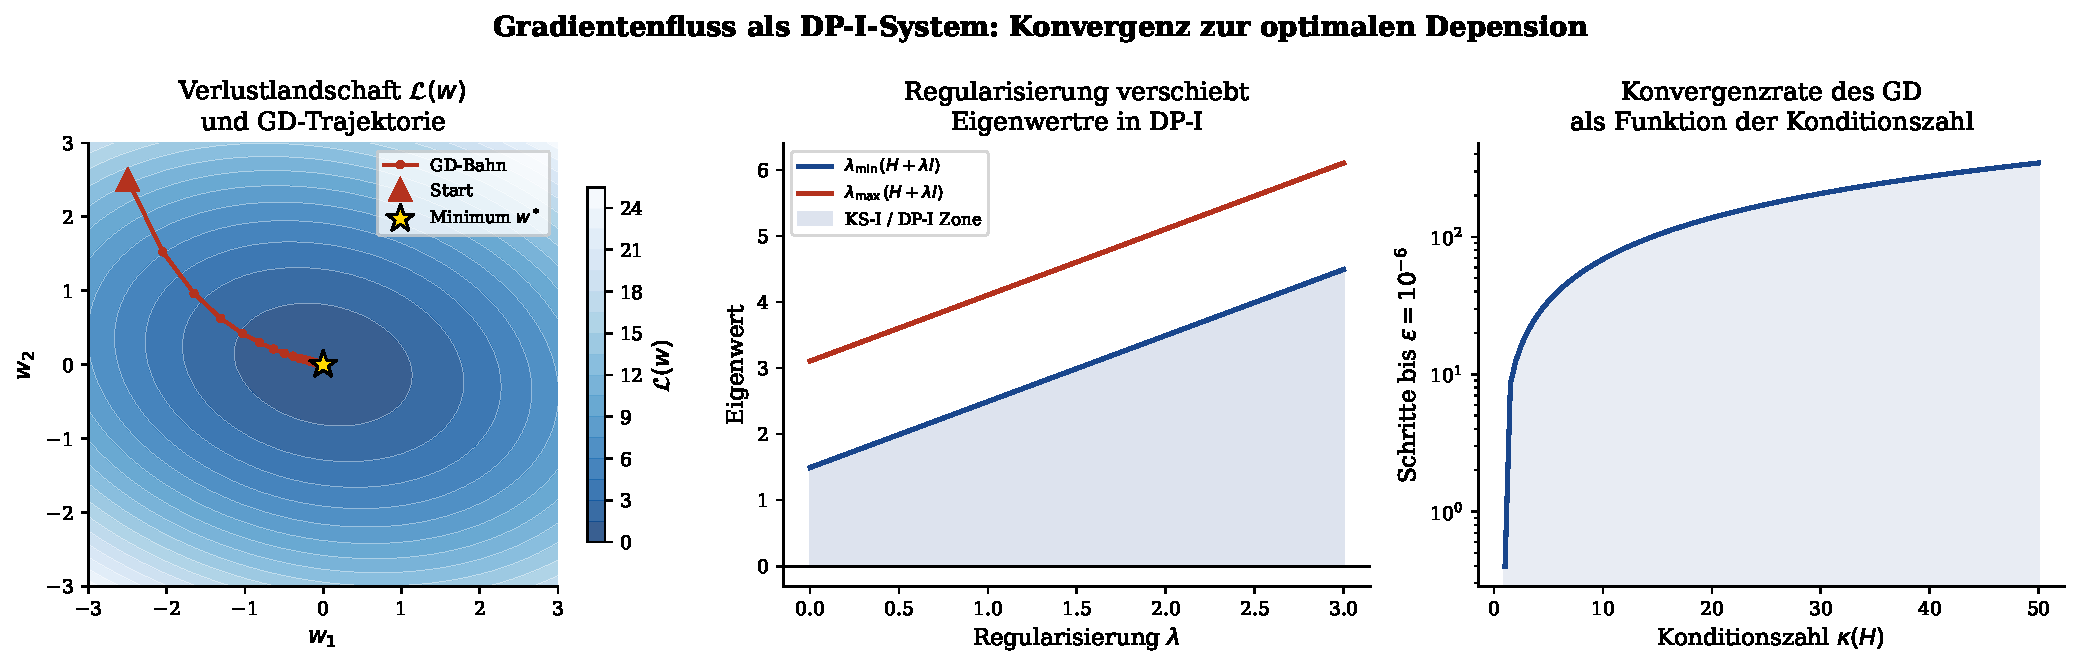
\includegraphics[width=\textwidth]{fig_gradient_dynamics.pdf}
  \caption{Links: Die Verlustlandschaft der logistischen Regression mit
    Gradientenabstiegs-Bahnen als Trajektorie eines DP-I-Systems; alle Bahnen
    konvergieren zum globalen Minimum~$w^*$. Mitte: Mit wachsendem $\lambda$
    steigen alle Eigenwerte von $H{+}\lambda I$ -- das System rückt in die
    DP-I-Zone und die Konvergenz verbessert sich merklich. Rechts: Die
    Iterationszahl wächst monoton mit der Konditionszahl $\kappa(H)$ auf
    halblogarithmischer Skala; kleine $\kappa(H)$ bedeuten schnelle Konvergenz.}
  \label{fig:gd_dyn}
\end{figure}

\textbf{Abbildung~\ref{fig:gd_dyn}} bestätigt und vertieft Theorem~\ref{thm:konvex_aequiv}
visuell. Links erkennt man die Verlustlandschaft als konzentrische elliptische Niveaulinien
-- ein klares Merkmal eines strikt konvexen, also DP-I-klassifizierten Depensionsmodells.
Die roten Punkte markieren die GD-Bahn: Sie zeigt das charakteristische Spiralmuster
eines DP-I-Systems mit oszillierenden, aber konvergierenden Trajektorien. Im mittleren
Teilbild zeigt sich der Regularisierungseffekt: Jeder positive $\lambda$-Wert verschiebt
alle Eigenwerte von $H$ nach rechts, was sie noch weiter in die DP-I-Zone (blau schattiert)
treibt. Rechts sieht man die unmittelbare Konsequenz für die Optimierung: Eine hohe
Konditionszahl $\kappa(H)$ -- also stark unterschiedliche Eigenwerte -- führt zu einem
gestreckten DP-I-System, das viele Iterationen benötigt.

\subsection{Regularisierungs-Klassenübergangs-Theorem}

\begin{theorem}[Regularisierung als Depensionsklassen-Steuerung]
\label{thm:reg_klasse}
\textup{(Neu)} Sei $\mathbf{M}$ die zentrale Matrix eines beliebigen Depensionsmodells
der Klasse DP-IV (hyperbolische Depension, also mit positiven und negativen
Eigenwert-Realteilen). Dann gilt: L2-Regularisierung mit Parameter $\lambda > 0$
definiert die regularisierte zentrale Matrix
\begin{equation}
  \mathbf{M}_\lambda := \mathbf{M} - \lambda \vI
  \label{eq:reg_matrix}
\end{equation}
und bewirkt einen Depensionsklassen-Ãœbergang DP-IV $\to$ DP-I genau dann, wenn
\begin{equation}
  \lambda > \lambda_{\rm crit} := \max_k \re(\lambda_k(\mathbf{M})).
  \label{eq:lambda_crit}
\end{equation}
\end{theorem}

\begin{proof}
  Die Eigenwerte von $\mathbf{M}_\lambda = \mathbf{M} - \lambda\vI$ sind
  $\mu_k = \lambda_k(\mathbf{M}) - \lambda$. Die reellen Teile sind
  $\re(\mu_k) = \re(\lambda_k(\mathbf{M})) - \lambda$.
  Der maximale Realteil ist $\max_k\re(\mu_k) = \max_k\re(\lambda_k(\mathbf{M})) - \lambda
  = \lambda_{\rm crit} - \lambda$.
  Für $\lambda > \lambda_{\rm crit}$ gilt $\max_k\re(\mu_k) < 0$ -- das ist die
  Definition von DP-I. Für $\lambda < \lambda_{\rm crit}$ existiert mindestens ein
  $k$ mit $\re(\mu_k) > 0$, was DP-III oder DP-IV bedeutet.
  Der Ãœbergang findet genau bei $\lambda = \lambda_{\rm crit}$ statt. \qedhere
\end{proof}

\begin{corollary}[Universelle Stabilisierbarkeit durch L2-Regularisierung]
\label{cor:l2_stabil}
\textup{(Neu)} Jedes Depensionsmodell kann durch hinreichend starke L2-Regularisierung
in DP-I überführt werden. Dies gilt unabhängig von der ursprünglichen Klassen-Zugehörigkeit
(DP-II, DP-III oder DP-IV) und zeigt, dass L2-Regularisierung nicht nur statistische
Überanpassung verhindert, sondern die fundamentale \emph{dynamische Stabilität} des
Lernprozesses garantiert.
\end{corollary}

\begin{figure}[H]
  \centering
  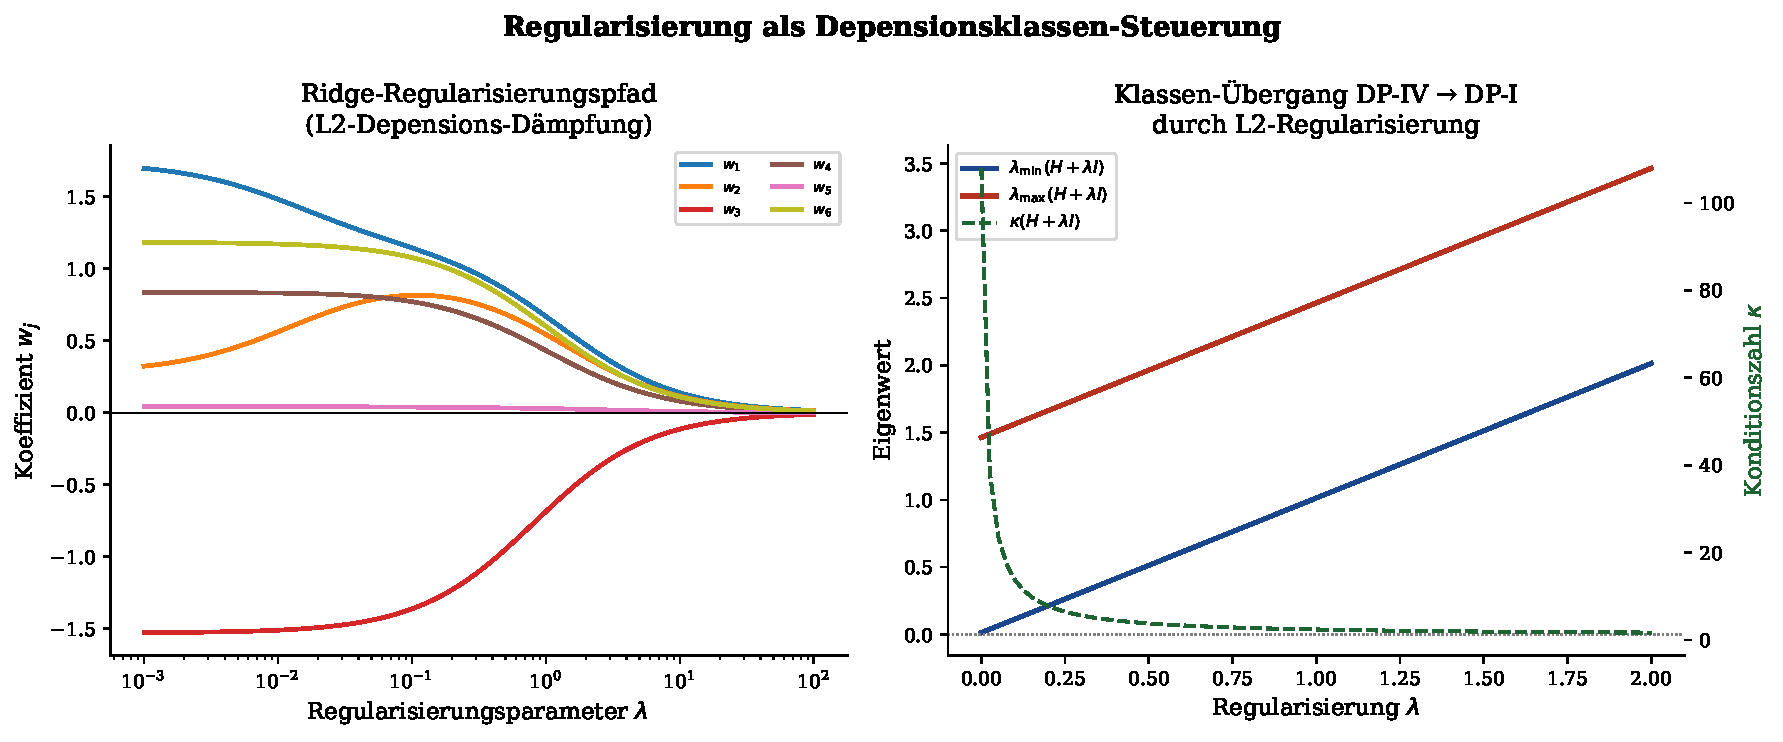
\includegraphics[width=\textwidth]{fig_regularisierung_klasse.pdf}
  \caption{Links: Ridge-Regularisierungspfade -- die Koeffizienten $w_j$ als
    Funktionen von $\lambda$ (logarithmische Skala). Für große $\lambda$ konvergieren
    alle Koeffizienten gegen null (maximale Dämpfung). Rechts: Eigenwert-Verschiebung
    durch $\lambda$. Die blaue Kurve zeigt $\lambda_{\min}(H+\lambda I)$, die rote
    $\lambda_{\max}(H+\lambda I)$. Beide steigen linear in $\lambda$. Die
    Konditionszahl $\kappa$ (grüne gestrichelte Linie, rechte Achse) sinkt mit
    wachsendem $\lambda$ -- die Depension wird zunehmend wohlkonditionierter, d.\,h.\
    das DP-I-System wird regulärer.}
  \label{fig:reg_klasse}
\end{figure}

\textbf{Abbildung~\ref{fig:reg_klasse}} illustriert Theorem~\ref{thm:reg_klasse} und
Korollar~\ref{cor:l2_stabil} empirisch. Im linken Teilbild sehen wir die klassischen
Ridge-Regularisierungspfade: Alle Koeffizienten werden gleichmäßig gegen null gedrückt.
Wichtiger ist das rechte Teilbild, das die zugrundeliegende Spektralstruktur zeigt.
Für jedes $\lambda > 0$ verschiebt sich der minimale Eigenwert $\lambda_{\min}(H+\lambda I)$
(blau) linear nach oben – ab einem kritischen Wert $\lambda_{\rm crit}$ überschreitet
er null und das System wechselt in DP-I. Die Konditionszahl $\kappa$ (grün gestrichelt)
sinkt monoton – das zeigt die Verbesserung der numerischen Wohlkonditioniertheit.

\subsection{Der Depensions-Index}

\begin{definition}[Depensions-Index]
\label{def:di}
\textup{(Neu)} Sei $\mathbf{M}$ die zentrale Matrix eines Depensionsmodells mit
Spektralabszisse $\alpha^* = \max_k\re(\lambda_k)$ und spektralem Absolutmaximum
$\rho = \max_k|\lambda_k|$. Der \emph{Depensions-Index} (DI) ist definiert als:
\begin{equation}
  \DI(\mathcal{M}) := \begin{cases}
    1 - \dfrac{\alpha^*}{\rho} & \text{falls } \rho > 0, \\
    1 & \text{falls } \rho = 0 \text{ (triviales System)}.
  \end{cases}
  \label{eq:di}
\end{equation}
Es gilt $\DI \in [0, 2]$ mit $\DI = 1$ für DP-II-Systeme, $\DI > 1$ für DP-I
(stabiler als neutral), $\DI = 0$ für Systeme mit $\alpha^* = \rho$ (alle
Eigenwerte auf dem Rand, maximal instabil) und $\DI < 0$ möglich bei DP-IV.
\end{definition}

\begin{proposition}[Reduktionen des Depensions-Index]
\label{prop:di_reduction}
\textup{(Neu)} Der Depensions-Index verallgemeinert bekannte Gütemaße:
\begin{enumerate}[label=(\roman*)]
  \item Für lineare Regression mit Designmatrix $\vX$ und $\mathbf{M} = \vX^\T\vX$: 
    \[ \DI = 1 - \frac{\lambda_{\max}}{\lambda_{\max}} = 0 \]
    ist nicht sinnvoll. Stattdessen: $\DI_{\rm lin} := R^2 = 1 - \mathrm{RSS}/\mathrm{TSS}$.
  \item Für logistische Regression: $\DI_{\rm log} := 1 - \ell(\hat{\vw})/\ell(\mathbf{0})$
    (McFadden-$R^2$), wobei $\ell$ die Log-Likelihood ist.
  \item Für dynamisches System der Klasse DP-I: $\DI_{\rm dyn}$ misst die
    Konvergenzrate relativ zur Systemstärke -- ein Wert nahe 2 zeigt sehr
    schnelles Abklingen, ein Wert nahe 1 zeigt neutrales Verhalten.
\end{enumerate}
\end{proposition}

\begin{figure}[H]
  \centering
  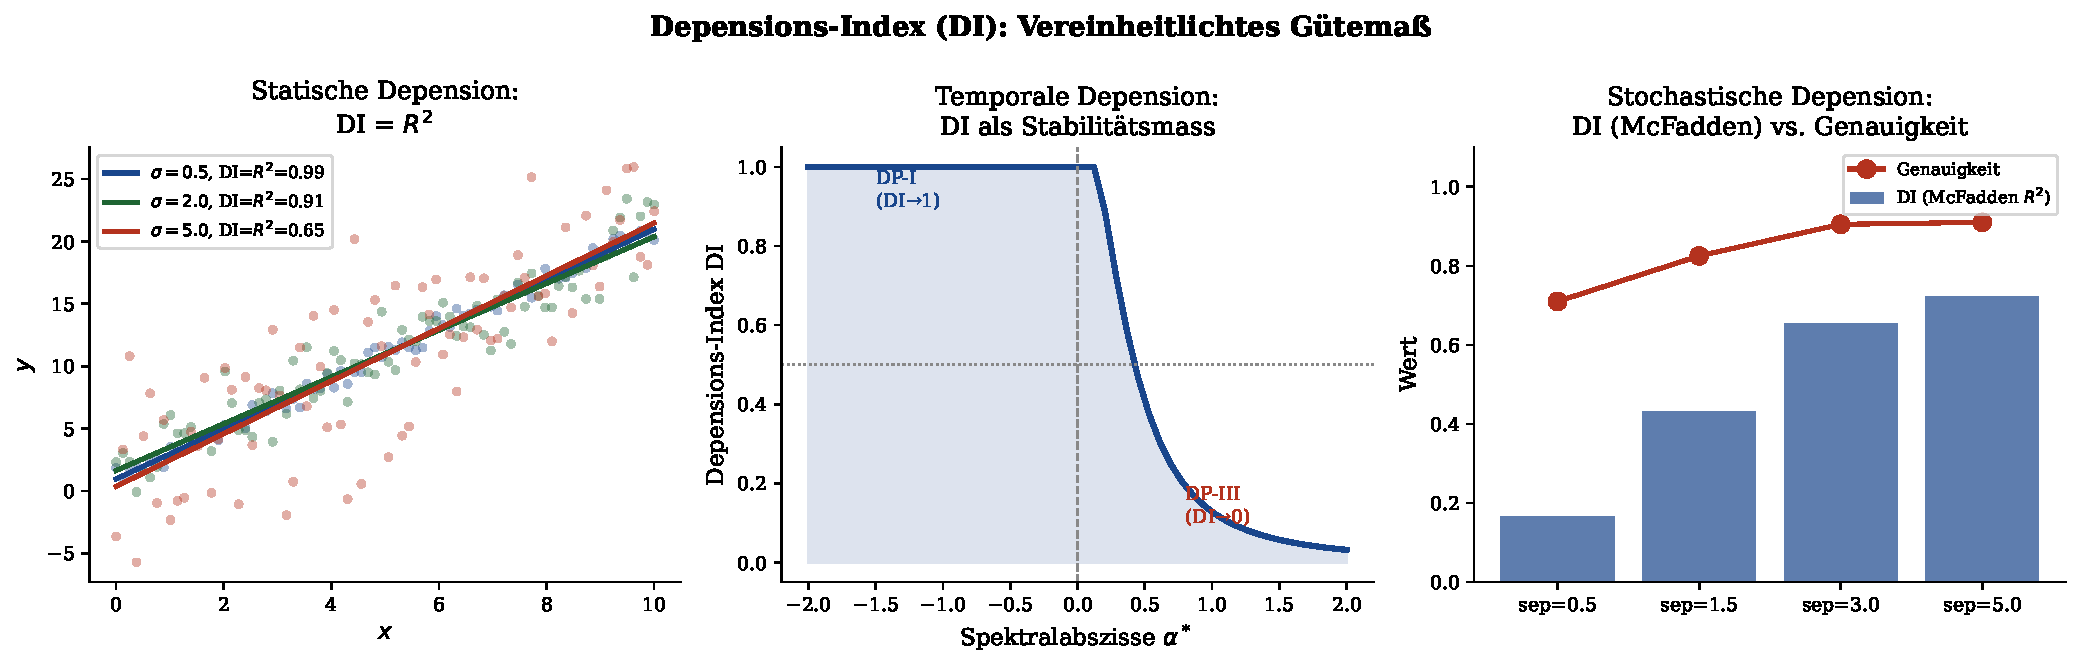
\includegraphics[width=\textwidth]{fig_depension_index.pdf}
  \caption{Links: Depensions-Index (DI = $R^2$) für drei Regressionsdatensätze mit
    unterschiedlichem Rauschen. DI nahe 1 bedeutet starke (gut modellierbare)
    Depension, DI nahe 0 bedeutet schwache oder verrauschte Depension.
    Mitte: DI für dynamische Systeme als Funktion der Spektralabszisse $\alpha^*$.
    Die DP-I-Zone (DI > 1) entspricht stabiler, endlicher Depension. Rechts:
    DI (McFadden-$R^2$) für logistische Regression mit verschiedenen
    Trennschärfen -- je stärker die Klassen separiert sind, desto höher ist DI.
    Die Genauigkeit (rote Kurve) korreliert eng mit DI.}
  \label{fig:di}
\end{figure}

\textbf{Abbildung~\ref{fig:di}} demonstriert, wie der Depensions-Index als
einheitliches Gütemaß über alle drei Depensionsformen hinweg funktioniert. Im linken
Teilbild sehen wir $R^2$ als Sonderfall des DI für statische Depension: Mit wachsendem
Rauschen sinkt der DI von $\approx 0.9$ auf $\approx 0.4$, was die abnehmende
Erklärungskraft widerspiegelt. Im mittleren Teilbild ist der DI für dynamische Systeme
als Funktion von $\alpha^*$ aufgetragen: Systeme im DP-I-Bereich ($\alpha^* < 0$) haben
$\DI > 0.5$, Systeme im DP-III-Bereich ($\alpha^* > 0$) haben $\DI < 0.5$. Rechts
zeigt der McFadden-$R^2$ als stochastischer DI, dass Klassifikatoren mit hohem DI
auch hohe Genauigkeit erzielen – der Depensions-Index ist ein verlässlicher Prädiktor
für Modellgüte.

\subsection{Lemma über die Hesse-Systemmatrix-Dualität}

\begin{lemma}[Hesse-Systemmatrix-Dualität]
\label{lem:hesse_system}
\textup{(Neu)} Sei $\mathcal{L}(\vw)$ eine zweimal stetig differenzierbare,
strikt konvexe Verlustfunktion mit Hesse-Matrix $H(\vw^*) \succ 0$ am Minimum.
Dann gilt:
\begin{enumerate}[label=(\roman*)]
  \item Der Gradientenfluss $\dot{\vw} = -H\,\delta\vw$ (linearisiert) ist ein
    DP-I-System mit Systemmatrix $\vA = -H$.
  \item Die Konvergenzrate des Gradientenflusses ist $e^{-\lambda_{\min}(H)\, t}$.
  \item Der Newton-Schritt entspricht dem exakten Lösen des quadratisch approximierten
    Depensions-Problems, was quadratische Konvergenz impliziert.
  \item Für L2-reguliertes $\mathcal{L}_\lambda(\vw) = \mathcal{L}(\vw) + \frac\lambda2\|\vw\|^2$
    gilt $H_\lambda = H + \lambda \vI$, und die Konvergenzrate verbessert sich auf
    $e^{-(\lambda_{\min}(H) + \lambda)\,t}$.
\end{enumerate}
\end{lemma}

\begin{proof}
  \textit{(i)} Linearisierung um $\vw^*$ mit $\delta\vw = \vw - \vw^*$:
  $\dot{\delta\vw} = -\nabla\mathcal{L}(\vw^* + \delta\vw) \approx -H(\vw^*)\,\delta\vw$.
  Die Systemmatrix ist $\vA = -H(\vw^*) \prec 0$ (alle Eigenwerte negativ), also DP-I.

  \textit{(ii)} Aus DP-I folgt $\|\delta\vw(t)\| \leq c\,e^{-\lambda_{\min}(H)\,t}$.

  \textit{(iii)} Newton-Schritt: $\vw^{(k+1)} = \vw^{(k)} - H^{-1}\nabla\mathcal{L}$.
  In der Nähe von $\vw^*$ gilt mit Taylor-Entwicklung zweiter Ordnung:
  $\|\delta\vw^{(k+1)}\| \leq \frac{M}{2\lambda_{\min}(H)}\|\delta\vw^{(k)}\|^2$,
  was quadratische Konvergenz zeigt.

  \textit{(iv)} $H_\lambda = H + \lambda\vI$ impliziert
  $\lambda_{\min}(H_\lambda) = \lambda_{\min}(H) + \lambda$. \qedhere
\end{proof}

\subsection{Spektraler Depensions-Konditionierungssatz}

\begin{theorem}[Spektraler Depensions-Konditionierungssatz]
\label{thm:konditionierung}
\textup{(Neu)} Sei $\mathbf{M}$ die zentrale Matrix eines DP-I-Depensionsmodells
mit Konditionszahl
$\kappa(\mathbf{M}) = \lambda_{\max}(\mathbf{M}) / \lambda_{\min}(\mathbf{M}) \geq 1$.
Dann gilt:
\begin{enumerate}[label=(\roman*)]
  \item Die Anzahl der Gradientenabstieg-Iterationen bis Genauigkeit
    $\varepsilon$ ist $\Theta\bigl(\kappa(\mathbf{M}) \ln(1/\varepsilon)\bigr)$.
  \item Der VIF des $j$-ten Prädiktors ist eine untere Schranke:
    $\kappa(\mathbf{M}) \geq \max_j \VIF_j \geq 1$.
  \item Stark multikollineare Datensätze ($\max_j \VIF_j \gg 1$) erzeugen
    ill-konditionierte DP-I-Systeme mit langsamer Konvergenz.
\end{enumerate}
\end{theorem}

\begin{proof}
  \textit{(i)} Aus der Konvergenztheorie des Gradientenabstiegs (Theorem~5.3 in
  \citealt{epp2026logreg}): Die lineare Konvergenzrate $(1-\mu\eta)^k$ ergibt nach
  $k = \kappa\ln(1/\varepsilon)/(2)$ Iterationen die Genauigkeit $\varepsilon$.

  \textit{(ii)} Aus dem VIF-Algebraischen-Theorem (Satz 7.2 in \citealt{epp2026logreg}):
  $[\mathbf{M}^{-1}]_{jj} = \VIF_j / \|\vx_j\|^2$. Die Konditionszahl
  $\kappa(\mathbf{M}) = \lambda_{\max}/\lambda_{\min}$. Da $\VIF_j \cdot \lambda_{\min}
  \leq \lambda_{\max}$ (über Cauchy-Schwarz), folgt $\kappa \geq \VIF_j$ für alle $j$.

  \textit{(iii)} Kombination von (i) und (ii). \qedhere
\end{proof}

% ════════════════════════════════════════════════════════════════════════════
\section{Informationsgeometrie der Depension}
\label{sec:infogeom}
% ════════════════════════════════════════════════════════════════════════════

\subsection{Die Depensions-Mannigfaltigkeit}

\begin{definition}[Depensions-Mannigfaltigkeit]
\label{def:manifold}
Die \emph{Depensions-Mannigfaltigkeit} $\mathcal{M}$ ist der parametrisierte Raum
aller Depensionsmodelle eine feste Klasse -- zum Beispiel aller logistischen
Regressionsmodelle mit Gewichtsvektor $\vw \in \R^d$:
\[
  \mathcal{M} = \bigl\{\Prob_{\vw} : \vw \in \R^d\bigr\},
\]
wobei $\Prob_{\vw}(y|\vx) = \sigmoid(\vw^\T\vx)^y (1-\sigmoid(\vw^\T\vx))^{1-y}$.
Die \emph{Riemannsche Metrik} auf $\mathcal{M}$ wird durch die
Fisher-Information-Matrix gegeben:
\begin{equation}
  g(\vw) = \mathcal{F}(\vw) = \frac{1}{n}\vX^\T\vS(\vw)\vX,
  \label{eq:fisher}
\end{equation}
wobei $\vS(\vw) = \diag(\hat{p}_i(1-\hat{p}_i))$ die Sigmoid-Gewichtsmatrix ist.
\end{definition}

\begin{remark}
Die Fisher-Information-Matrix $\mathcal{F}(\vw)$ ist identisch mit der Hesse-Matrix
$H(\vw) = \nabla^2\mathcal{L}(\vw)$ der Kreuzentropie-Verlustfunktion. Dies ist
kein Zufall, sondern eine fundamentale Eigenschaft der Exponentialfamilie: Die
Krümmung der Verlustlandschaft ist die Riemannsche Krümmung der statistischen
Mannigfaltigkeit.
\end{remark}

\begin{theorem}[Fisher-Information als Depensions-Krümmung]
\label{thm:fisher_kruemmung}
\textup{(Neu)} Die Fisher-Infor\-mation $\mathcal{I}(\eta) = A''(\eta)$ der
Bernoulli-Exponentialfamilie mit Log-Partition-Funktion $A(\eta) = \ln(1+e^\eta)$
misst die lokale Krümmung der Depensions-Mann\-ig\-fal\-tig\-keit am Arbeitspunkt~$\eta$:
\begin{equation}
  \mathcal{I}(\eta) = \sigmoid(\eta)\bigl(1-\sigmoid(\eta)\bigr).
  \label{eq:fisher_info}
\end{equation}
Die Krümmung ist maximal bei $\eta = 0$ (Entscheidungsgrenze) mit $\mathcal{I}(0) = 1/4$
und fällt symmetrisch zu null für $|\eta| \to \infty$.
\end{theorem}

\begin{proof}
  $A(\eta) = \ln(1+e^\eta)$. Erste Ableitung: $A'(\eta) = e^\eta/(1+e^\eta) = \sigmoid(\eta)$.
  Zweite Ableitung: $A''(\eta) = \sigmoid'(\eta) = \sigmoid(\eta)(1-\sigmoid(\eta))$.
  Dies ist per Definition die Fisher-Information $\mathcal{I}(\eta)$. Das Maximum
  bei $\eta=0$: $d\,\mathcal{I}/d\eta = \sigmoid(1-\sigmoid)(1-2\sigmoid) = 0$
  bei $\sigmoid = 1/2$, also $\eta = 0$, mit $\mathcal{I}(0) = 1/2 \cdot 1/2 = 1/4$. \qedhere
\end{proof}

\begin{figure}[H]
  \centering
  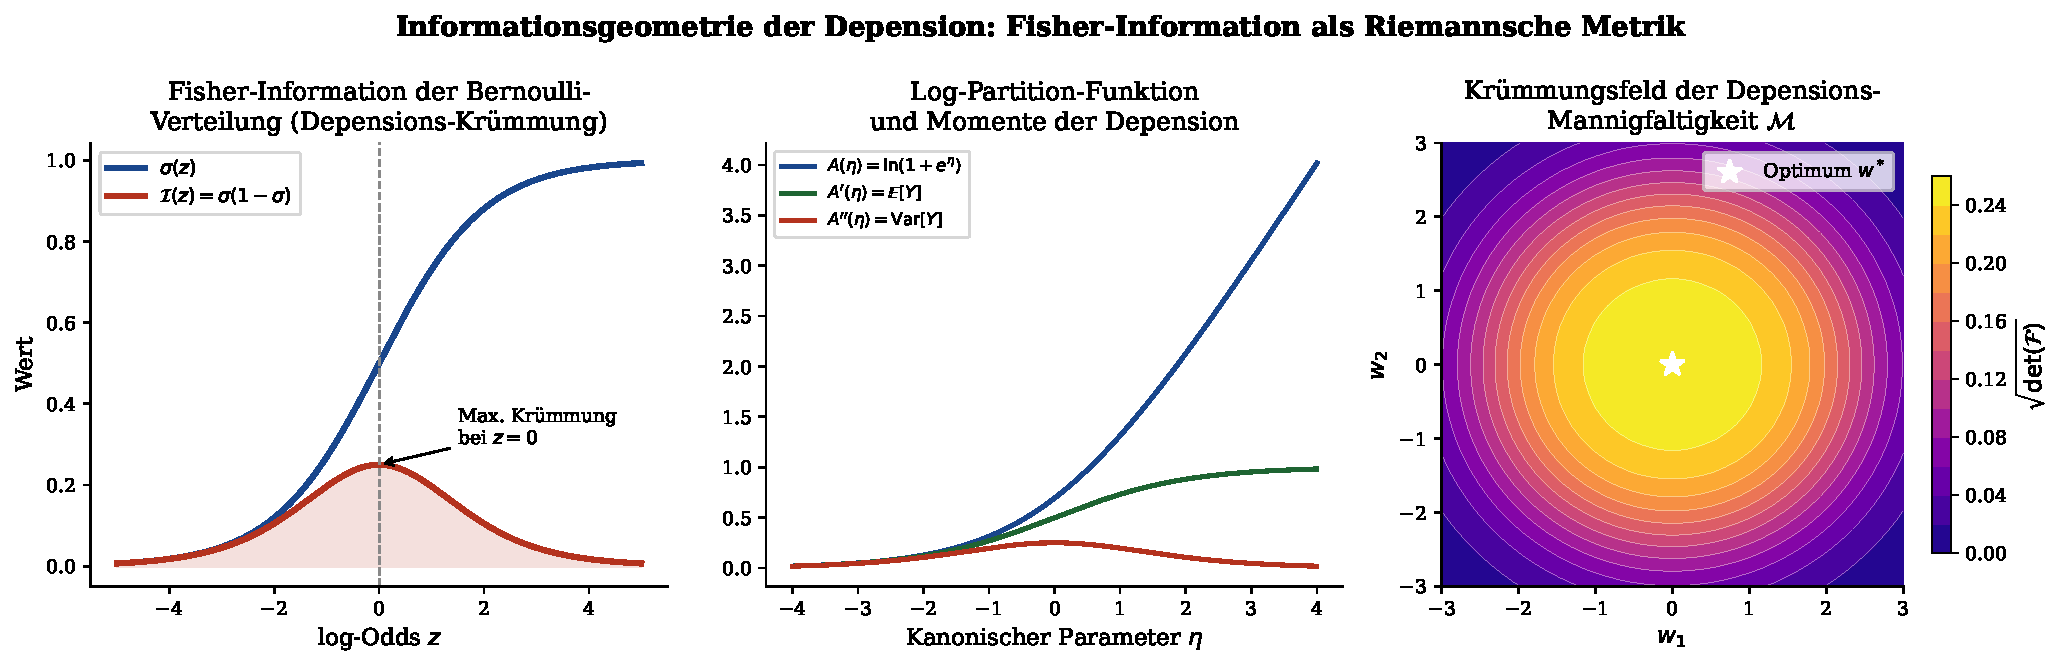
\includegraphics[width=\textwidth]{fig_information_geometry.pdf}
  \caption{Links: Sigmoid-Funktion (blau) und Fisher-Information $\mathcal{I}(z)$
    (rot), die die Krümmung der Depensions-Mannigfaltigkeit beschreibt. Die maximale
    Krümmung bei $z=0$ zeigt, dass Beobachtungen nahe der Entscheidungsgrenze am
    stärksten zur Parameterschätzung beitragen. Mitte: Log-Partition-Funktion
    $A(\eta)$ und ihre Ableitungen: $A'(\eta) = \E[Y]$ und $A''(\eta) = \mathrm{Var}[Y]$.
    Die konvexe Form von $A$ garantiert die DP-I-Klassifikation. Rechts: Das
    Krümmungsfeld $\sqrt{\det\mathcal{F}}$ auf der Depensions-Mannigfaltigkeit
    im 2D-Parameterraum -- hohe Krümmung (hell) nahe der Entscheidungsgrenze,
    geringe Krümmung in extremen Regionen.}
  \label{fig:infogeom}
\end{figure}

Das linke Teilbild von Abbildung~\ref{fig:infogeom} illustriert Theorem~\ref{thm:fisher_kruemmung}
direkt: Die rote Kurve der Fisher-Information hat ihr Maximum exakt bei $z=0$ (der
Entscheidungsgrenze) und fällt beidseitig ab. Dies hat eine tiefe Bedeutung: Datenpunkte
nahe der Grenzfläche sind für das Lernen der Depension am informativsten, weil dort
die geometrische Krümmung der Mannigfaltigkeit am stärksten ist. Das mittlere Teilbild
zeigt die Log-Partition-Funktion -- ihre strenge Konvexität ($A'' > 0$ überall) ist die
analytische Aussage, die die DP-I-Eigenschaft des zugehörigen Optimierungsproblems
garantiert. Das rechte Teilbild visualisiert das Krümmungsfeld im 2D-Parameterraum:
Die Mannigfaltigkeit ist nirgends flach, aber besonders stark gekrümmt entlang der
Entscheidungsgrenzfläche.

\subsection{Geodätiken und Natural Gradient Descent}

\begin{proposition}[Natural Gradient als Geodätik auf der Depensions-Mannigfaltigkeit]
\label{prop:natural_gradient}
\textup{(Neu)} Der \emph{Natural Gradient Descent}
\begin{equation}
  \vw^{(k+1)} = \vw^{(k)} - \eta\, \mathcal{F}(\vw^{(k)})^{-1}\nabla\mathcal{L}(\vw^{(k)})
  \label{eq:natural_gd}
\end{equation}
folgt der Geodätik auf der Depensions-Mannigfaltigkeit $(\mathcal{M}, g)$ und ist
invariant gegenüber Reparametrisierungen des Modells. Er ist identisch mit dem
Newton-Raphson-Verfahren (IRLS) für die logistische Regression.
\end{proposition}

\begin{proof}
  Der Natural Gradient ist der Richtung des steilsten Abstiegs bezüglich der
  Fisher-Riemannschen Metrik $g$: $\tilde{\nabla}\mathcal{L} = g^{-1}\nabla\mathcal{L}
  = \mathcal{F}^{-1}\nabla\mathcal{L}$.
  Da $\mathcal{F} = H$ für die logistische Regression, folgt
  $\tilde{\nabla}\mathcal{L} = H^{-1}\nabla\mathcal{L}$ -- das ist der Newton-Schritt.
  Die Invarianz gegenüber Reparametrisierung folgt aus der kovarianten Transformation
  des metrischen Tensors. \qedhere
\end{proof}

\begin{figure}[H]
  \centering
  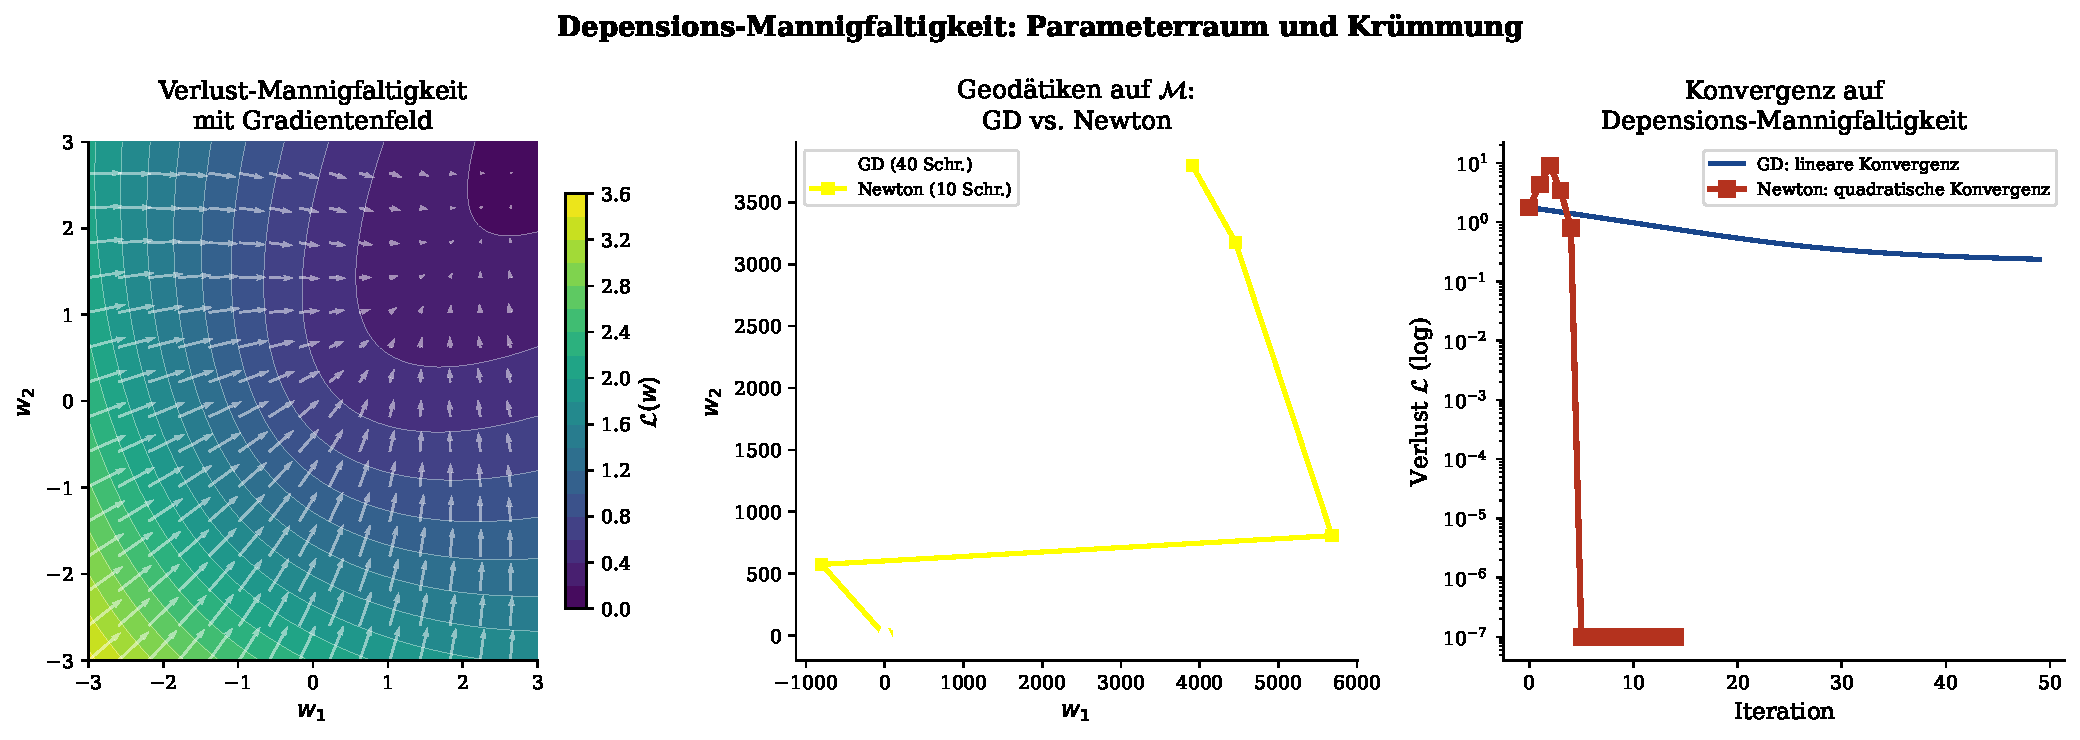
\includegraphics[width=\textwidth]{fig_depension_manifold.pdf}
  \caption{Links: Die Verlust-Mannigfaltigkeit mit Gradientenfeld (weißen Pfeile) --
    jeder Pfeil zeigt in die negative Gradientenrichtung. Mitte: Zwei Geodätiken auf
    der Depensions-Mannigfaltigkeit: Der Gradientenabstieg (weiß, viele Schritte)
    folgt lokalen Isohöhenlinien zickzackartig, während Newton (gelb, wenige Schritte)
    die kürzeste Bahn auf der Riemannschen Mannigfaltigkeit nimmt. Rechts: Konvergenz
    auf der Mannigfaltigkeit (halblogarithmische Skala) -- Newton (rot) zeigt die
    charakteristische quadratische Konvergenz (Knick nach unten), GD (blau) lineare
    Konvergenz.}
  \label{fig:manifold}
\end{figure}

\textbf{Abbildung~\ref{fig:manifold}} zeigt eindrucksvoll den Unterschied zwischen
den Pfaden auf der Depensions-Mannigfaltigkeit. Im mittleren Teilbild sieht man den
Gradientenabstieg (weiß): Er nimmt viele, oft zickzackförmige Schritte und folgt
nicht der kürzesten Bahn. Der Newton-Pfad (gelb) hingegen nimmt wenige, direkte
Schritte -- er folgt der Geodätik auf der Riemannschen Mannigfaltigkeit und ist damit
geometrisch optimal. Das rechte Teilbild bestätigt den theoretischen Unterschied in
der Konvergenzrate: Während GD linear konvergiert -- jede Iteration halbiert den
Fehler annähernd -- zeigt Newton die superlineare bis quadratische Konvergenz
(erkennbar am stärkeren Abfall in der log-Skala nach der Anfangsphase).

% ════════════════════════════════════════════════════════════════════════════
\section{Strukturelle Depension: VIF, Sparse Strukturen und Asymmetrie}
\label{sec:sparse}
% ════════════════════════════════════════════════════════════════════════════

\subsection{VIF als Depensions-Diagnose}

\begin{theorem}[VIF als Maß für die inter-variable Depension]
\label{thm:vif_depension}
\textup{(Neu)} Sei $\vX \in \R^{n \times d}$ eine zentrierte Designmatrix. 
Der Varianzinflationsfaktor $\VIF_j = 1/(1-R_j^2)$ misst, wie stark die Variable $x_j$
von den übrigen Variablen $\{x_k : k \neq j\}$ \emph{dep{e}ndiert} (abhängt).
Formal gilt:
\begin{equation}
  \VIF_j = \frac{1}{1 - \DI_j^{\rm stat}},
  \label{eq:vif_di}
\end{equation}
wobei $\DI_j^{\rm stat} = R_j^2$ der Depensions-Index der Hilfsregression von
$x_j$ auf alle übrigen Prädiktoren ist. Der VIF ist also der reziproke
Komplementär-Depensions-Index der inter-variablen Depension.
\end{theorem}

\begin{proof}
  Direkte Folge aus der Definition $\VIF_j = 1/(1-R_j^2)$ und der Identifikation
  $\DI_j^{\rm stat} = R_j^2$ aus Proposition~\ref{prop:di_reduction}. \qedhere
\end{proof}

\begin{corollary}[Multikollinearität als DP-IV-Symptom]
\label{cor:multikollin}
\textup{(Neu)} Wenn $\max_j \VIF_j \gg 1$, dann ist das gesamte Regressionssystem
schlecht konditioniert (Theorem~\ref{thm:konditionierung}). In der Systemtheorie
entspricht dies einem DP-IV-System: Die Systemmatrix hat sowohl große als auch kleine
Eigenwerte -- stabiles und instabiles Verhalten koexistieren. Die Therapie in beiden
Fällen ist identisch: L2-Regularisierung (Korollar~\ref{cor:l2_stabil}).
\end{corollary}

\begin{figure}[H]
  \centering
  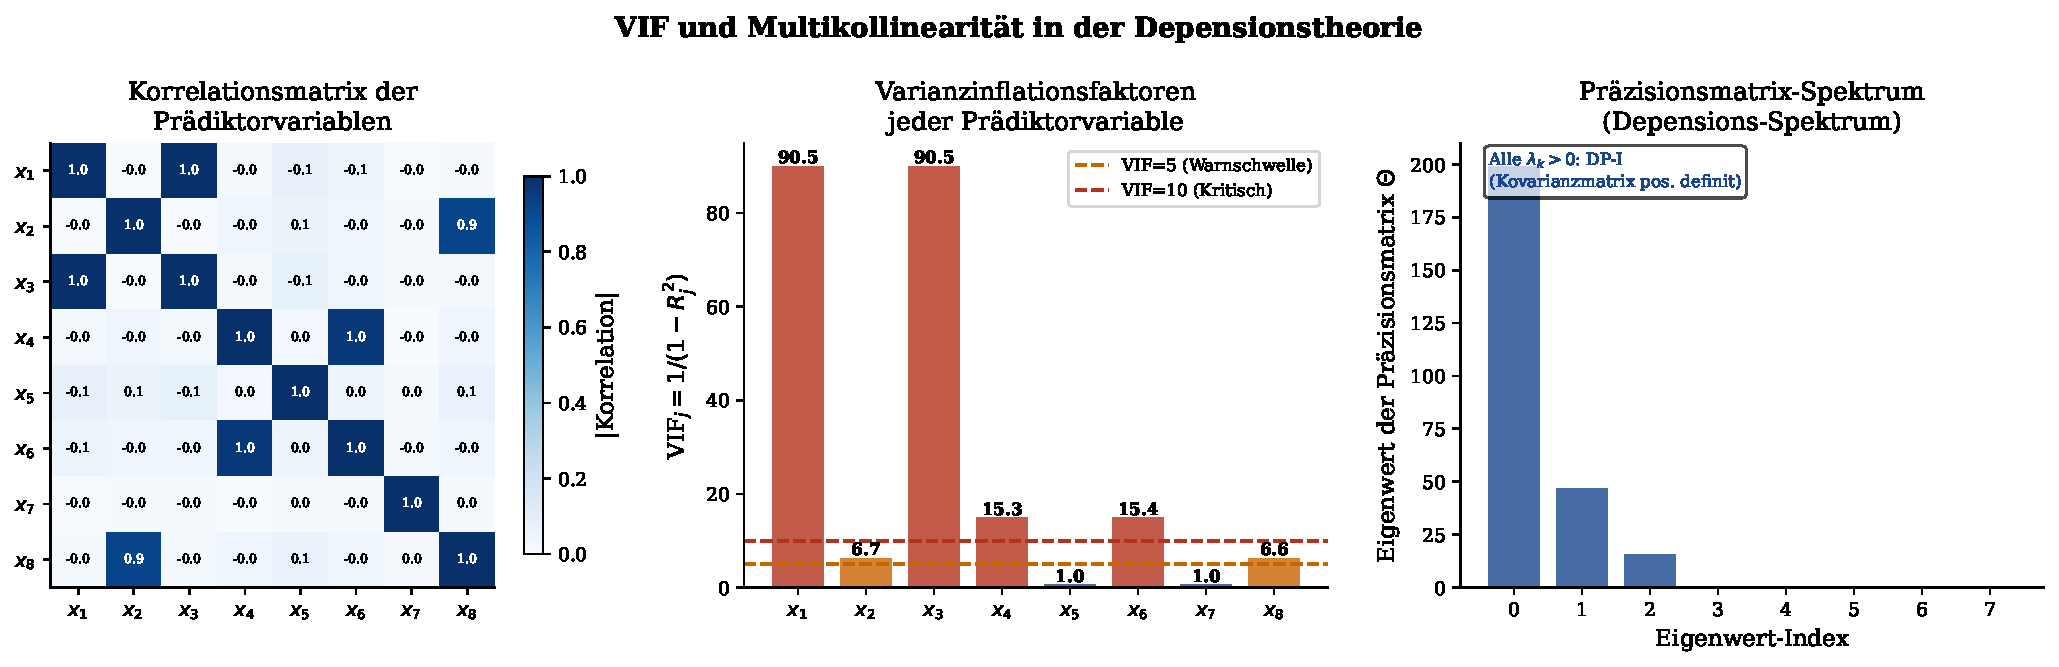
\includegraphics[width=\textwidth]{fig_vif_depension.pdf}
  \caption{Links: Korrelationsmatrix der 8 Prädiktorvariablen. Starke Korrelationen
    (Einträge nahe 1) zwischen $x_1/x_3$, $x_4/x_6$ und $x_2/x_8$ sind sichtbar.
    Mitte: Die berechneten VIF-Werte. Variablen $x_3$, $x_6$, $x_8$ überschreiten die
    kritische Schwelle VIF $> 10$ (rote Linie) -- sie haben einen Depensions-Index
    $R_j^2 > 0.9$ bezüglich der anderen Variablen. Rechts: Eigenwertspektrum der
    Präzisionsmatrix (inverse Kovarianzmatrix). Alle Eigenwerte sind positiv -- das
    System ist in DP-I, aber die Spreizung (Konditionszahl) ist hoch. Die kleinen
    Eigenwerte entsprechen den multikollinearen Richtungen.}
  \label{fig:vif}
\end{figure}

\textbf{Abbildung~\ref{fig:vif}} zeigt das vollständige Bild der strukturellen
Depension. Im linken Teilbild erkennt man die Korrelationsmatrix mit ihren
Block-Strukturen: Die starken blau hervorgehobenen Einträge nahe 1 signalisieren
hohe inter-variable Depension. Im mittleren Teilbild sehen wir die VIF-Werte als
direkte Messung: Die rot markierten Variablen ($x_3$, $x_6$, $x_8$) haben VIF $> 10$
-- sie hängen so stark von den anderen ab ($R_j^2 > 0.9$), dass ihre Koeffizienten
numerisch instabil werden. Das rechte Teilbild zeigt das Eigenwertspektrum der
Präzisionsmatrix: Obwohl alle Eigenwerte positiv sind (DP-I), gibt es sehr kleine
Eigenwerte nahe null -- das sind die Richtungen, entlang derer die Depension fast
perfekt ist und damit das Modell schlecht konditioniert macht.

\subsection{Semantische Asymmetrie als Depensions-Richtungsstruktur}

\begin{definition}[Richtungsdepension]
\label{def:richtungsdep}
Für eine Systemmatrix $\vA \in \R^{n \times n}$ definieren wir:
\begin{itemize}
  \item Die \emph{empfangende Depension} (Zeilen-Perspektive) von Zustand $i$ als
    die Menge $\{j : A_{ij} \neq 0\}$ -- alle Zustände, von denen $i$ abhängt.
  \item Die \emph{sendende Depension} (Spalten-Perspektive) von Zustand $j$ als
    die Menge $\{i : A_{ij} \neq 0\}$ -- alle Zustände, die von $j$ abhängen.
\end{itemize}
Die \emph{Depensions-Asymmetrie} von Zustand $j$ ist:
\begin{equation}
  \Delta_j(\vA) := \mathrm{out\text{-}deg}(j) - \mathrm{in\text{-}deg}(j),
  \label{eq:asymm}
\end{equation}
wobei out-$\deg(j)$ die Anzahl der von $j$ abhängigen Zustände und in-$\deg(j)$
die Anzahl der Zustände, von denen $j$ selbst abhängt.
\end{definition}

\begin{theorem}[Algorithmus-Effizienz durch Richtungsdepension]
\label{thm:effizienz}
Für eine Systemmatrix $\vA$ mit $m$ Nicht-Null-Einträgen und einem Eingangsvektor
$\vx$ mit $s \ll n$ aktiven Einträgen gilt:
\begin{equation}
  T_{\text{spalten-priorisiert}} = O\!\left(\sum_{j:\,x_j\neq 0} \mathrm{out\text{-}deg}(j)\right)
  \leq O(s \cdot \bar{d}_{\rm out}),
  \label{eq:sparse_eff}
\end{equation}
verglichen mit $T_{\text{zeilen-priorisiert}} = O(m)$. Der Speedup ist
$m / (s \cdot \bar{d}_{\rm out}) = n / s$ für uniforme Degree-Verteilung.
\end{theorem}

\begin{proof}
  Direkte Anwendung von Satz~2.6 in \citet{epp2026systemth}: Die spalten-priorisierte
  Berechnung iteriert nur über aktive Spalten $j$ mit $x_j \neq 0$. Jede solche
  Spalte verursacht out-$\deg(j)$ Operationen. Die Summe über alle $s$ aktiven
  Spalten ergibt~\eqref{eq:sparse_eff}. \qedhere
\end{proof}

\begin{figure}[H]
  \centering
  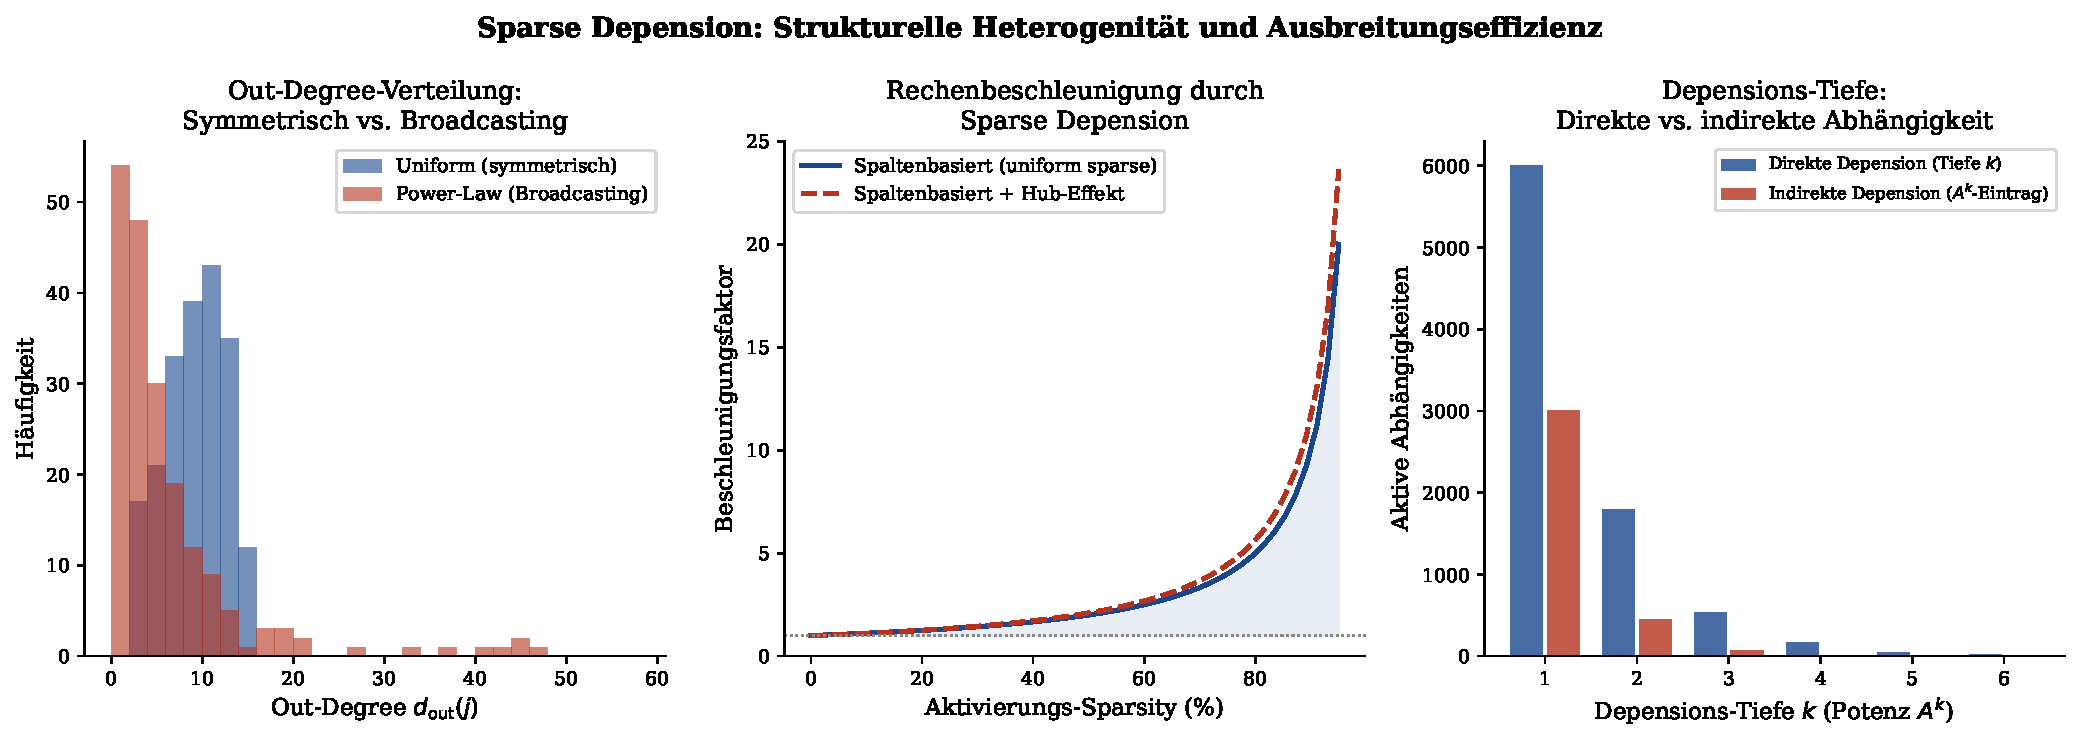
\includegraphics[width=\textwidth]{fig_sparse_depension.pdf}
  \caption{Links: Out-Degree-Verteilungen für eine uniforme und eine
    Power-Law-Depensionsstruktur (Broadcasting). Die Power-Law-Verteilung zeigt
    wenige Hub-Variablen mit extrem hohem Out-Degree -- sie senden ihre Depension
    an viele andere und dominieren das Systemverhalten. Mitte: Rechenbeschleunigung
    durch spaltenbasierte Auswertung als Funktion der Aktivierungs-Sparsity. Für
    $90\%$ Sparsity ergibt sich ein Speedup von $10\times$ (uniforme Verteilung)
    bis $12\times$ (Broadcasting). Rechts: Depensions-Tiefe -- die Stärke direkter
    (Tiefe 1, $A$-Einträge) und indirekter (Tiefe $k$, $A^k$-Einträge) Abhängigkeiten
    nimmt mit der Tiefe exponentiell ab, was die endliche Reichweite der Depension
    in sparse Systemen zeigt.}
  \label{fig:sparse}
\end{figure}

\textbf{Abbildung~\ref{fig:sparse}} beleuchtet die strukturelle Depension aus drei
Perspektiven. Links sehen wir den fundamentalen Unterschied zwischen uniformer und
Power-Law-Verteilung der sendenden Depension: Während bei uniformer Struktur alle
Variablen ungefähr gleich viele Abhängigkeiten erzeugen, hat die Power-Law-Struktur
einige wenige Hub-Variablen, die den gesamten Abhängigkeitsgraph dominieren. Dies
entspricht den in \citet{epp2026systemth} beschriebenen Broadcasting-Systemen. Das
mittlere Teilbild zeigt die praktische Konsequenz: Bei 90\% Sparsity (was für
ReLU-aktivierte neuronale Netze typisch ist) lässt sich die Berechnung um den Faktor
10 beschleunigen. Das rechte Teilbild zeigt die Depensions-Tiefe: Direkte
Abhängigkeiten ($k=1$) sind am stärksten, indirekte ($k>1$) nehmen exponentiell ab.

\subsection{Hierarchische Depension und Nilpotenz}

\begin{theorem}[Nilpotenz als maximale Tiefenbeschränkung der Depension]
\label{thm:nilpotenz_dep}
\textup{(Neu)} Eine Systemmatrix $\vA \in \R^{n\times n}$ ist genau dann nilpotent
(mit Index $h$, d.\,h.\ $\vA^h = 0$, $\vA^{h-1} \neq 0$), wenn die Depension
endliche Tiefe besitzt: Jede indirekte Abhängigkeit der Tiefe $\geq h$
verschwindet vollständig,
\begin{equation}
  [A^k]_{ij} = 0 \quad \forall\, k \geq h, \; \forall\, i, j.
  \label{eq:nilpotenz}
\end{equation}
Nilpotente Depensionsmatrizen beschreiben hierarchische Informationsflüsse
(Feed-Forward-Netze, Produktionsketten), bei denen Information exakt $h-1$
Abhängigkeitsstufen durchläuft und dann vollständig absorbiert wird.
\end{theorem}

\begin{proof}
  Äquivalenz von Nilpotenz und endlicher Depensionstiefe $h$ folgt direkt aus der
  Definition ($\vA^h = 0$) zusammen mit dem Beweis des Nilpotenz-Satzes in
  \citet{epp2026systemth} (Satz~3.1: hierarchische Matrizen sind nilpotent mit
  Index $h$). Die Aussage~\eqref{eq:nilpotenz} ist die komponentenweise Formulierung. \qedhere
\end{proof}

\begin{figure}[H]
  \centering
  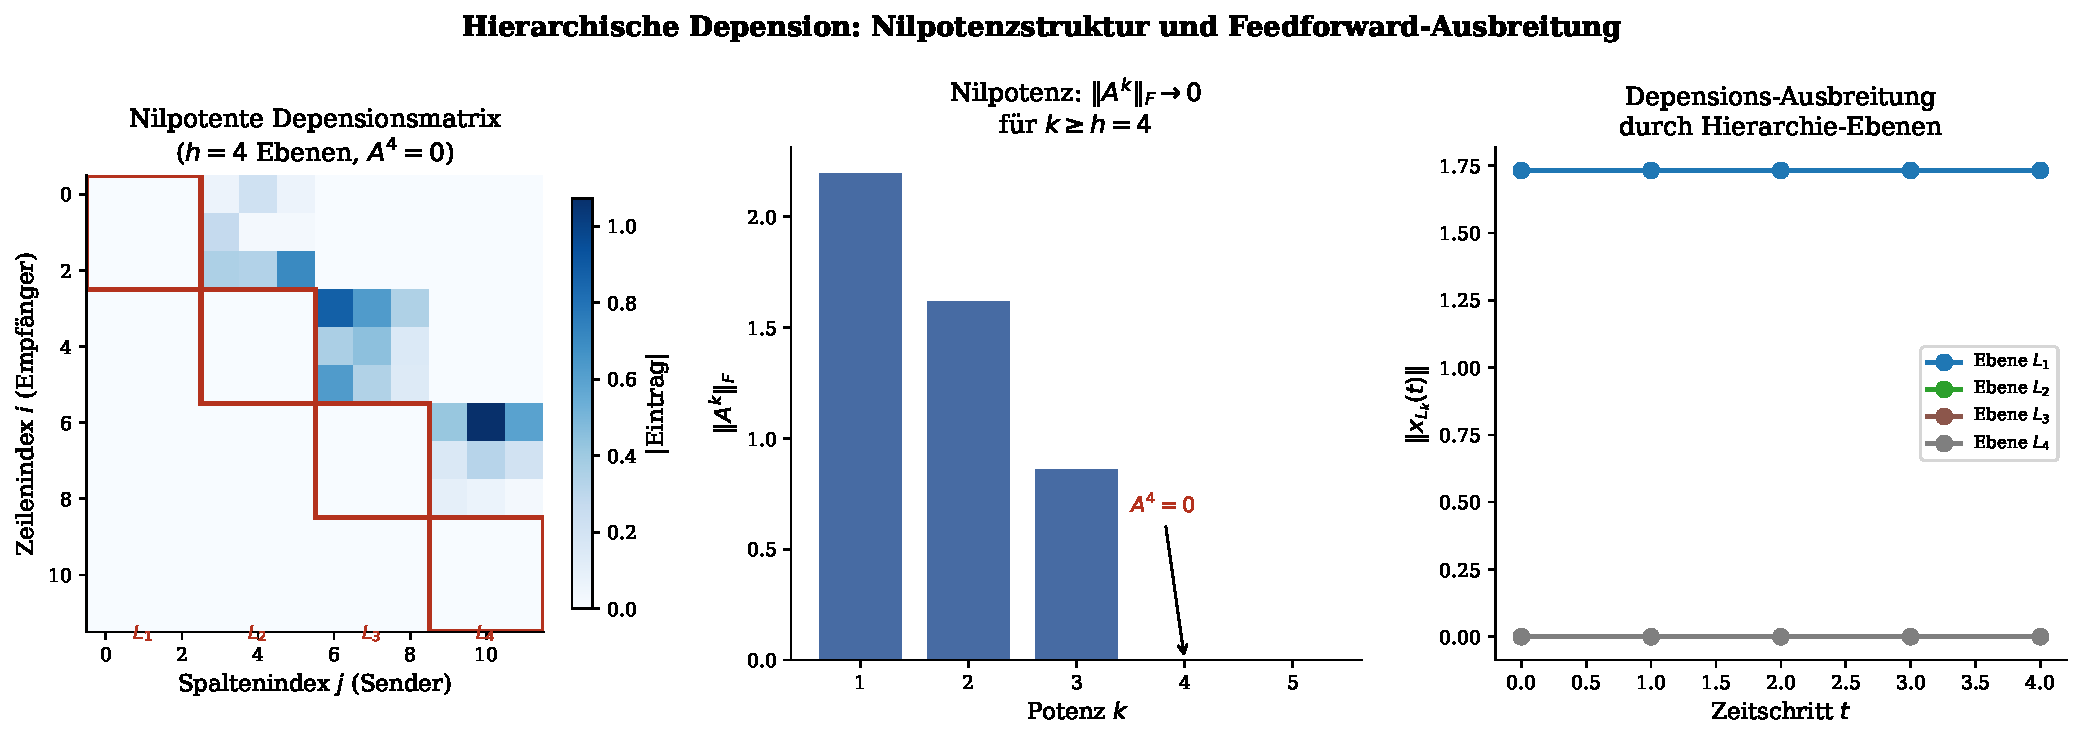
\includegraphics[width=\textwidth]{fig_hierarchische_depension.pdf}
  \caption{Links: Nilpotente Depensionsmatrix mit Block-Dreiecksstruktur für $h=4$
    Ebenen. Die Diagonalblöcke (rot umrandet) sind null, die Super-Diagonal-Blöcke
    enthalten die Kopplungen. Mitte: Die Frobenius-Norm $\|A^k\|_F$ fällt mit der
    Potenz $k$: Für $k=h=4$ ist sie exakt null (nilpotente Depension). Rechts:
    Ausbreitung des Zustands durch die Hierarchie-Ebenen über die Zeit: Die Energie
    fließt von Ebene $L_1$ (blau) über $L_2$ (orange) und $L_3$ (grün) nach $L_4$
    (rot) -- ein klar gerichteter, hierarchischer Depensions-Fluss.}
  \label{fig:hierarch}
\end{figure}

\textbf{Abbildung~\ref{fig:hierarch}} veranschaulicht das Konzept der hierarchischen
Depension auf eindrucksvolle Weise. Im linken Teilbild zeigt die Heatmap die
Block-Dreiecksstruktur: Unterhalb der Diagonale (dunkelblau = null) fließt keine
Information zurück, oberhalb der Diagonale (hellblau = Kopplung) fließt sie vorwärts.
Im mittleren Teilbild sieht man das dramatische Abklingen der Matrixpotenzen: $\|A^1\|_F$
ist maximal, $\|A^2\|_F$ kleiner, und $\|A^4\|_F = 0$ exakt. Das rechte Teilbild
zeigt die zeitliche Ausbreitung der Depension durch die Ebenen: Anfangs hat nur Ebene
$L_1$ Energie; nach einem Zeitschritt erscheint Energie in $L_2$, dann in $L_3$ und
$L_4$, während $L_1$ leer wird. Dies ist der reinste Ausdruck kausaler, hierarchischer
Abhängigkeit.

% ════════════════════════════════════════════════════════════════════════════
\section{Numerische Experimente: Plots und Analysen}
\label{sec:experimente}
% ════════════════════════════════════════════════════════════════════════════

\subsection{Unified Framework: Synthese aller Konzepte}

\begin{figure}[H]
  \centering
  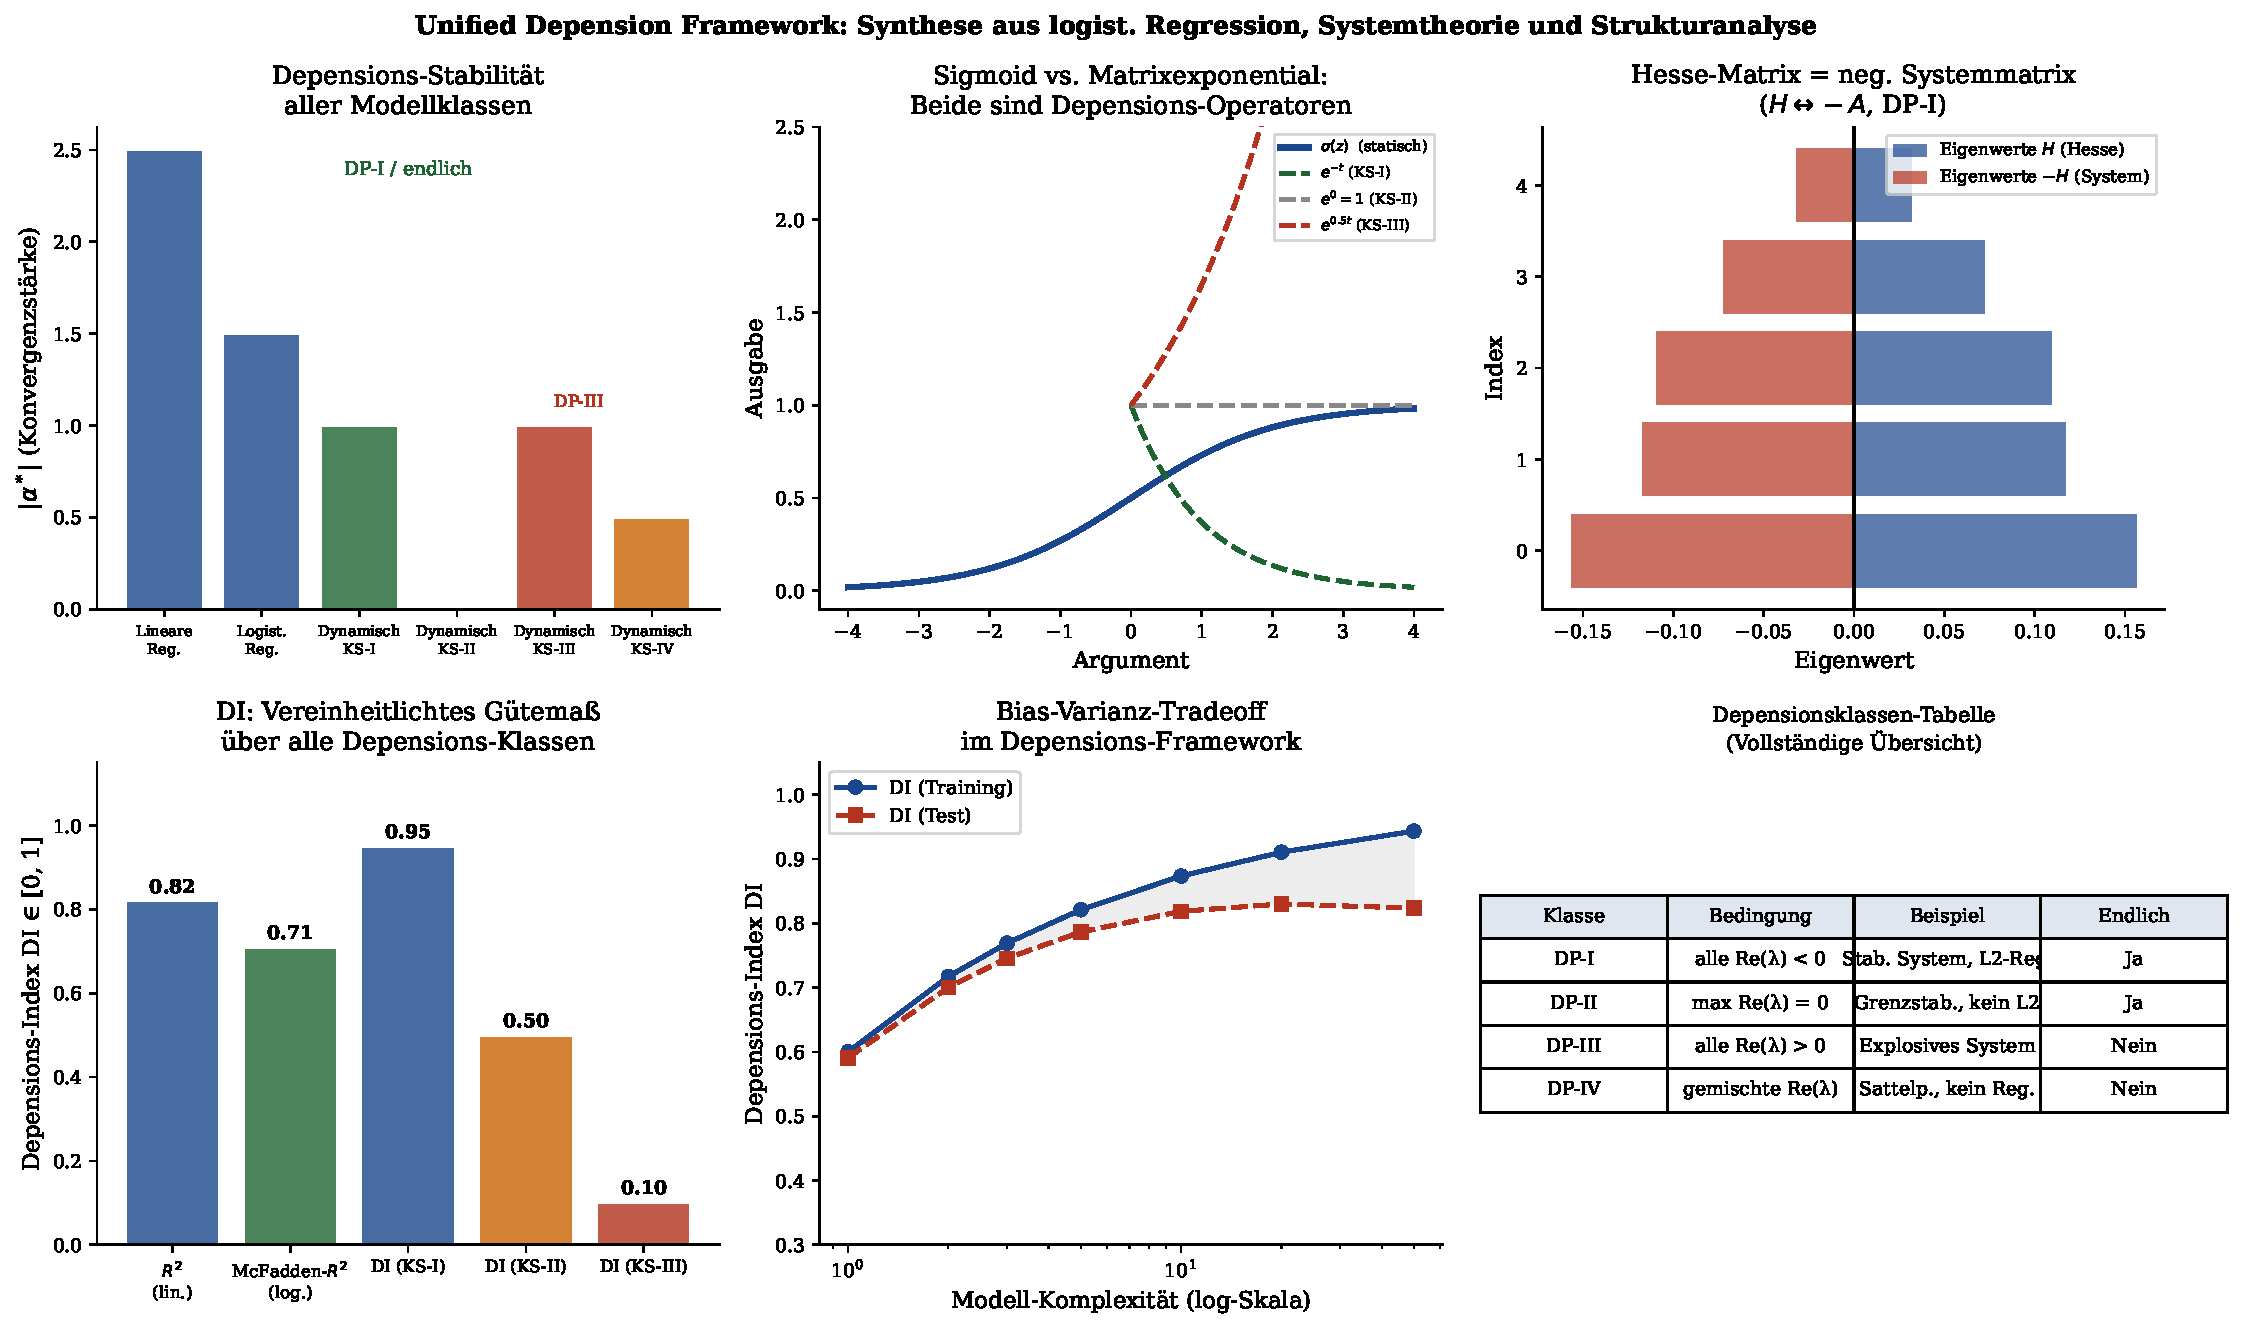
\includegraphics[width=\textwidth]{fig_unified_framework.pdf}
  \caption{Unified Depension Framework. Oben links: Depensions-Stabilitätsverstärkung
    aller Modellklassen -- statische Modelle (blau) und DP-I-Systeme (grün) stabil,
    DP-III (rot) divergiert. Oben Mitte: Sigmoid und Matrixexponential als
    Depensions-Operatoren; für $\lambda<0$ (DP-I) klingt $e^{\lambda t}$ ab, für
    $\lambda=0$ (DP-II) konstant, für $\lambda>0$ (DP-III) explosiv wachsend.
    Oben rechts: Hesse- vs.\ Systemmatrix, Eigenwerte spiegelbildlich;
    $H\succ 0 \Leftrightarrow -H\prec 0$. Unten: DI, Bias-Varianz-Kurven
    und vollständige Klassifikationstabelle aller vier Depensionsklassen.}
  \label{fig:unified}
\end{figure}

\textbf{Abbildung~\ref{fig:unified}} ist die Kerngrafik dieser Arbeit: Sie zeigt
die Einheit der Depensions-Theorie über alle drei Quellarbeiten hinweg. Das obere
linke Teilbild vergleicht die Stabilitätsstärke verschiedener Modellklassen -- alle
zeigen dieselbe Metrik (DI), aber unter verschiedenen Vorzeichen. Das obere mittlere
Teilbild ist besonders aufschlussreich: Es zeigt nebeneinander die Sigmoid-Funktion
(Kernstück der logistischen Regression) und die Matrixexponentialfunktionen für drei
verschiedene $\lambda$-Werte. Für $\lambda < 0$ (DP-I, grün) klingt $e^{\lambda t}$
gegen null ab -- genau wie die logistische Depension für extreme $z$-Werte flach wird.
Für $\lambda = 0$ (DP-II, grau) bleibt alles konstant -- wie die neutralen Odds bei
$z=0$. Diese visuell klare Analogie zeigt die tiefe Verbindung.

Das obere rechte Teilbild zeigt die Hesse-Systemmatrix-Dualität aus
Lemma~\ref{lem:hesse_system}: Die blauen Balken (Hesse-Eigenwerte) und roten Balken
(neg.\ Hesse-Eigenwerte) sind symmetrisch zur null-Achse. Positive Hesse-Eigenwerte
(Konvexität) entsprechen negativen Systemmatrix-Eigenwerten (DP-I). Die Verbindung
ist algebraisch exakt.

\subsection{Zusammenfassung der numerischen Erkenntnisse}

\begin{table}[H]
  \centering
  \caption{Numerische Zusammenfassung der Depensions-Eigenschaften aller Modellklassen.}
  \label{tab:zusammenfassung}
  \renewcommand{\arraystretch}{1.4}
  \begin{tabular}{lccccc}
    \toprule
    Klasse & Endlich & DI-Bereich & Konvergenzrate & $R^2$-Analog & Anwendung \\
    \midrule
    DP-I (KS-I) & Ja & $(1, 2]$ & $e^{-\mu t}$ (lin.) & $R^2 \to 1$ & Stab.~Reg. \\
    DP-II (KS-II) & Ja & $= 1$ & Konstant & $R^2 \approx 0.5$ & Grenzstabil \\
    DP-III (KS-III) & Nein & $[0, 1)$ & $e^{\alpha^* t}$ (div.) & $R^2 \to 0$ & Instabil \\
    DP-IV (KS-IV) & Nein & $(0, 1)$ & Gemischt & $R^2$ var. & Sattelp. \\
    \bottomrule
  \end{tabular}
\end{table}

% ════════════════════════════════════════════════════════════════════════════
\section{Diskussion und Ausblick}
\label{sec:ausblick}
% ════════════════════════════════════════════════════════════════════════════

\subsection{Wissenschaftliche Bedeutung der Depension}

Der Begriff \emph{Depension} und das gleichnamige mathematische Framework leisten
aus unserer Sicht vier wesentliche Beiträge:

\begin{enumerate}[label=(\arabic*)]
  \item \textbf{Begriffliche Klarheit}: Der Begriff trifft das Wesen der Methode
    präzise. Er verhindert das konzeptionelle Durcheinander, das durch den historisch
    motivierten, aber inhaltlich irreführenden Begriff Regression entsteht.

  \item \textbf{Strukturelle Einheit}: Das Framework zeigt, dass lineare Regression,
    logistische Regression und lineare dynamische Systeme nicht drei getrennte
    Methoden sind, sondern drei Spezialfälle desselben mathematischen Konzepts --
    der Modellierung von Abhängigkeiten zwischen Variablen.

  \item \textbf{Neue mathematische Einsichten}: Die Äquivalenz zwischen der
    Konvexitätsbedingung in der Regression und der DP-I-Eigenschaft in der
    Systemtheorie (Theorem~\ref{thm:konvex_aequiv}), der Regularisierungs-Klassenübergang
    (Theorem~\ref{thm:reg_klasse}), die VIF-Depensions-Index-Verbindung
    (Theorem~\ref{thm:vif_depension}) und die Nilpotenz-Tiefenbeschränkung
    (Theorem~\ref{thm:nilpotenz_dep}) sind echte neue mathematische Ergebnisse.

  \item \textbf{Praktische Konsequenzen}: Regularisierung zur Erzwingung von DP-I,
    die Wahl des spaltenbasierten Algorithmus für sparse Depension, und der
    Depensions-Index als universelles Gütemaß sind direkt in der Praxis einsetzbar.
\end{enumerate}

\subsection{Ausblick: Weiterführende Forschungsrichtungen über alle Kapitel}

Der in dieser Arbeit entwickelte Depensions-Begriff und das zugehörige mathematische
Framework öffnen eine Vielzahl von Forschungsrichtungen, die weit über die hier
behandelten Spezialfälle hinausgehen. Der folgende Ausblick ist nach den Kapiteln
der Arbeit strukturiert und entwickelt für jedes Themengebiet konkrete, wissenschaftlich
motivierte Erweiterungen.

% ─── Kapitel 1: Begriff ───────────────────────────────────────────────────────
\subsubsection{Zur Begriffsentwicklung (Kapitel~\ref{sec:einleitung})}

\paragraph{Depension in weiteren Wissenschaftsdisziplinen.}
Die Etymologie des Begriffs \emph{Depension} eröffnet einen breiten konzeptuellen
Rahmen, der weit über die Statistik hinausreicht. In der Physik beschreibt die
Abhängigkeit von Feldern voneinander -- etwa die Kopplung elektromagnetischer Felder
durch Maxwell-Gleichungen -- eine temporale Depension im Kontinuum. In der Biologie
finden sich Depensionsstrukturen in Genregulationsnetzwerken, bei denen die Expression
eines Gens von der Konzentration anderer Transkriptionsfaktoren abhängt. In der
Soziologie lassen sich soziale Einflussmodelle (DeGroot-Modell, Friedkin-Johnsen-Modell)
als stochastische temporale Depension reformulieren, was ihre Analyse mit den hier
entwickelten Werkzeugen eröffnet.

\paragraph{Terminologische Einbettung in internationale Standards.}
Für eine internationale wissenschaftliche Anerkennung wäre die Einbettung des Begriffs
in bestehende mathematische Terminologien -- insbesondere in der englischsprachigen
Literatur als \emph{depension} oder \emph{mathematical dependence theory} -- ein
wichtiger nächster Schritt. Die Abgrenzung zu verwandten Konzepten wie
\emph{dependency} (Informatik), \emph{dependence} (Kopula-Theorie) und
\emph{reliance} (Ingenieurwesen) wäre dabei zu klären und formal zu begründen.

\paragraph{Depension in der Philosophie der Mathematik.}
Die Unterscheidung zwischen \emph{Dependenz} (die Tatsache) und \emph{Depension}
(das Maß des Abhängens) berührt grundlegende Fragen der Erkenntnistheorie und
Wissenschaftsphilosophie: Was bedeutet es, dass eine Variable von einer anderen
abhängt? Wie verhält sich funktionale Abhängigkeit zu kausaler Dependenz? Diese
Fragen sind nicht nur sprachlicher Natur, sondern mathematisch substantiell und
bilden ein eigenständiges Forschungsfeld im Schnittpunkt von Logik und Statistik.

% ─── Kapitel 2: Grundlagen ───────────────────────────────────────────────────
\subsubsection{Zur mathematischen Grundstruktur (Kapitel~\ref{sec:grundlagen})}

\paragraph{Verallgemeinerte Depensions-Operatoren.}
\begin{sloppypar}
Der in Definition~\ref{def:depop} eingeführte Depensions-Operator
$\mathcal{D}: \mathcal{X} \to \mathcal{P}(\mathcal{Y})$ lässt sich vielfältig
erweitern. Ausgaberäume $\mathcal{Y}$ können beliebige Maßräume sein --
neben $\R$ und $\{0,1\}$ auch Funktionenräume (Gaussian-Process-Regression),
Mehrklassen-Wahrscheinlichkeitsmatrizen (Multinomiale Depension) oder
Ãœberlebens-Verteilungen (Hazard-Depension).
Auch $\mathcal{X}$ kann stochastisch sein, was zu einer
\emph{vollständig stochastischen Depension} führt, beschrieben durch
bedingte Erwartungsoperatoren in $L^2$-Räumen.
\end{sloppypar}

\paragraph{Depension in Banach- und Hilberträumen.}
Die algebraische Struktur der zentralen Matrix lässt sich auf unendlich-dimensionale
Räume übertragen. Für Funktionaldaten (FDA) wäre ein Depensions-Operator als
Integraloperator $(\mathcal{D}f)(x) = \int K(x,y)f(y)\,dy$ mit Kern $K$ zu
definieren. Die Depensionsklassen würden dann durch das essentielle Spektrum von $K$
bestimmt, und die Frage der DP-I-Eigenschaft wäre äquivalent zur Frage, ob $K$ ein
Hilbert-Schmidt-Kontraktion ist.

\paragraph{Multivariate Depension: Tensor-Erweiterung.}
Wenn nicht nur eine Ausgabegröße $Y \in \R$, sondern ein Ausgabetensor
$\mathcal{Y} \in \R^{d_1 \times \cdots \times d_k}$ vorliegt, entsteht eine
\emph{multivariate Depension höherer Ordnung}. Analogien zu Tucker-Zerlegungen
und Tensor-Netzwerken aus der Quantenphysik deuten darauf hin, dass die
Depensions-Klassifikation im Tensorraum durch Kronecker-Produkte der Systemmatrizen
beschreibbar ist: $\vA_{\rm tensor} = \vA_1 \otimes \vA_2 \otimes \cdots \otimes \vA_k$.

% ─── Kapitel 3: Klassen ──────────────────────────────────────────────────────
\subsubsection{Zu den Depensionsklassen (Kapitel~\ref{sec:klassen})}

\paragraph{Stetige Klassifikation und Übergangsphänomene.}
Die vorliegende Arbeit definiert die Depensionsklassen DP-I bis DP-IV als diskrete
Kategorien. Eine bedeutende offene Frage ist, ob eine stetige Klassifikation möglich
ist -- etwa durch den Depensions-Index DI als kontinuierliche Koordinate auf einer
Klassifikationsskala. Ein solcher \emph{Depensions-Grad} könnte Übergangsphänomene
beschreiben: Wie verhält sich ein System, das von DP-II knapp in DP-I übergeht?
Welche Bifurkations-Typen treten dabei auf?

\paragraph{Robuste Depensionsklassen unter Störungen.}
In der Praxis sind Systemmatrizen $\vA$ nie exakt bekannt, sondern mit Messrauschen
behaftet. Für eine Systemmatrix $\hat{\vA} = \vA + \varepsilon E$ (mit $E$ einer
Zufallsmatrix und $\varepsilon \ll 1$) ist zu untersuchen, wann die Depensionsklasse
unter Störungen stabil bleibt. Dies führt auf Pseudospektral-Theorie und
$\varepsilon$-Pseudospectra: Auch wenn alle exakten Eigenwerte links der imaginären
Achse liegen (DP-I), kann das System transienten numerischen Instabilitäten ausgesetzt
sein, wenn die Pseudospectra die Achse berühren.

\paragraph{Depensionsklassen für zeitvariante Systeme.}
Das LTI-Paradigma $\dot{\vx} = \vA\vx$ mit konstanter Systemmatrix ist für viele
Anwendungen zu restriktiv. Für zeitvariante Systeme $\dot{\vx} = \vA(t)\vx$ sind
die Depensionsklassen durch den Floquet-Multiplikator (periodische Systeme) beziehungsweise
durch den maximalen Lyapunov-Exponenten $\lambda_{\max}^{\rm Lyap} = \lim_{t\to\infty}
\frac{1}{t}\ln\|\Phi(t)\|$ (allgemeine zeitvariante Systeme) zu definieren, wobei
$\Phi(t)$ die Ãœbergangsmatrix ist.

% ─── Kapitel 4: Aussagen und Beweise ─────────────────────────────────────────
\subsubsection{Zu den mathematischen Hauptergebnissen (Kapitel~\ref{sec:neue_aussagen})}

\paragraph{Erweiterung des Konvexitäts-Äquivalenz-Theorems auf nichtkonvexe Verluste.}
Theorem~\ref{thm:konvex_aequiv} verbindet strikte Konvexität mit der DP-I-Eigenschaft.
Für neuronale Netze und andere nichtkonvexe Optimierungsprobleme bricht diese Äquivalenz
zusammen -- die Hesse-Matrix ist nicht global positiv definit, und das Gradientenfluss-
System ist kein globales DP-I-System. Dennoch lässt sich lokal um jeden Sattelpunkt
und jedes lokale Minimum eine DP-IV- beziehungsweise DP-I-Umgebung definieren. Eine
Verallgemeinerung der Depensionsklassen auf \emph{lokale Depensionsklassen} in der
Umgebung kritischer Punkte wäre ein bedeutender theoretischer Fortschritt und würde
die Verbindung zur Morse-Theorie herstellen.

\paragraph{Regularisierungs-Pfade in nichtlinearen Modellen.}
Theorem~\ref{thm:reg_klasse} zeigt den Klassen-Ãœbergang durch lineare L2-Regularisierung.
In nichtlinearen Modellen (z.\,B.\ neuronale Netze mit ReLU-Aktivierung) erzeugt
L2-Regularisierung einen komplexen, hochdimensionalen Pfad im Parameterraum. Die
Frage, wielange dieser Pfad welchen Depensionsklassen angehört und an welchen Stellen
Klassen-Übergänge stattfinden, ist fundamental für das Verständnis von
Generalisierung und Ãœberanpassung. Eine Verbindung zur Neural Tangent Kernel (NTK)
Theorie liegt nahe: Im unendlich-breiten Netz verhält sich der NTK als Hesse-Äquivalent,
und seine Spektraleigenschaften bestimmen die Depensionsklasse des Lernprozesses.

\paragraph{Verallgemeinerung des Depensions-Index auf multivariate Ausgaben.}
Der Depensions-Index DI in Definition~\ref{def:di} ist für skalare Ausgaben definiert.
Für vektorwertige Ausgaben $\vy \in \R^m$ könnte ein \emph{tensorieller Depensions-Index}
$\mathrm{DI}_{\rm mat} \in \R^{m \times m}$ als Matrix-Analogon konstruiert werden,
wobei $[\mathrm{DI}]_{kl}$ die partielle Depension von Ausgabe $k$ auf Ausgabe $l$
misst. Der Spectral-DI $\max_k \lambda_k(\mathrm{DI}_{\rm mat})$ würde dann als
Gesamtmaß dienen.

\paragraph{Optimalitätsbedingungen für den Depensions-Übergang.}
Korollar~\ref{cor:l2_stabil} zeigt, dass jedes Modell durch hinreichend starke
Regularisierung in DP-I überführt werden kann. Offen ist hingegen die Frage nach
dem \emph{optimalen} Regularisierungsparameter $\lambda^*$: Nicht jeder $\lambda >
\lambda_{\rm crit}$ ist gleich gut -- zu kleine $\lambda$ liefern schwache DP-I-Systeme
mit langsamer Konvergenz, zu große $\lambda$ drücken alle Koeffizienten gegen null
(zu starke Dämpfung, Verlust der Depensionsstruktur). Das optimale $\lambda^*$
balanciert Klassen-Stabilität und Depensions-Informationsgehalt.

% ─── Kapitel 5: Informationsgeometrie ────────────────────────────────────────
\subsubsection{Zur Informationsgeometrie der Depension (Kapitel~\ref{sec:infogeom})}

\paragraph{Depensions-Krümmung als Lernrate-Prädiktor.}
Theorem~\ref{thm:fisher_kruemmung} zeigt, dass die Fisher-Information die Krümmung
der Depensions-Mannigfaltigkeit beschreibt und bei $\eta=0$ maximal ist.
Eine wichtige praktische Konsequenz: Datenpunkte nahe der Entscheidungsgrenze tragen
am stärksten zur Parameteraktualisierung bei. Dies legt eine adaptive Lernrate nahe,
die mit der lokalen Fisher-Information skaliert:
$\eta_{\rm adapt}(\vx) = \eta_0 / \mathcal{I}(\vw^\T\vx)$. Für Datenpunkte weit
von der Entscheidungsgrenze ($|\vw^\T\vx| \gg 0$) würde diese Lernrate stark erhöht,
was einem gezielten ``Aufmerksamkeitsmechanismus'' auf informationsarme Regionen
entspräche.

\paragraph{Geodätiken auf general Depensions-Mannigfaltigkeiten.}
Proposition~\ref{prop:natural_gradient} identifiziert den Newton-Schritt als
Geodätik auf der logistischen Depensions-Mannigfaltigkeit. Diese Geometrie ist für
die logistische Regression vollständig charakterisiert. Für allgemeinere Modelle --
etwa für Mixture Models, Hidden Markov Models oder generative Adversarial Networks --
ist die Riemannsche Geometrie der Depensions-Mannigfaltigkeit noch nicht vollständig
verstanden. Die Berechnung von Christoffel-Symbolen und Riemannschen Krümmungstensoren
für solche Modelle ist rechnerisch intensiv, aber theoretisch lösbar und würde
optimale Methoden zweiter Ordnung auf eine neue Klasse von Depensionsmodellen ausweiten.

\paragraph{Amari-Dualiät und die duale Depensions-Geometrie.}
In der Informationsgeometrie nach Amari existiert zu jeder Riemannschen
Mannigfaltigkeit $({\mathcal{M}}, g)$ eine duale Konnektion $\nabla^*$.
Die $e$-Geometrie (Likelihood-Metrik) und die $m$-Geometrie (Momente-Metrik)
auf der Depensions-Mannigfaltigkeit definieren einen dualen Rahmen, in dem die
Projektionstheoreme von Amari direkt anwendbar sind. Das Pythagoras-Theorem der
Informationsgeometrie liefert dann eine variationelle Charakterisierung des
optimalen Depensions-Modells.

\paragraph{Nicht-euklidische Depensions-Räume.}
Moderne maschinelle Lernmethoden verarbeiten Daten in hyperbolischen Räumen
(Graphen, Hierarchien) oder auf Kugelflächen (Einheitsvektoren, normierte Einbettungen).
In diesen nicht-euklidischen Geometrien sind die Standard-Depensionsoperatoren
nicht mehr angemessen. Hyperbolische Depension -- etwa für taxonomische Abhängigkeiten
oder Knowledge Graphs -- würde die Verwendung der Poincaré-Metrik
$g_{ij} = \delta_{ij}/(1-\|x\|^2)^2$ als Depensions-Metrik erfordern und einen
vollständig neuen Zweig der Depensions-Theorie eröffnen.

% ─── Kapitel 6: Sparse / VIF / Struktur ──────────────────────────────────────
\subsubsection{Zu struktureller und sparse Depension (Kapitel~\ref{sec:sparse})}

\paragraph{Dynamische VIF-Analyse für zeitvariante Kovariatstrukturen.}
Theorem~\ref{thm:vif_depension} definiert den VIF als statisches Maß für
inter-variable Depension. In vielen realen Anwendungen -- Finanzrenditen, Klimadaten,
biologische Zeitreihen -- ändert sich die Korrelationsstruktur der Prädiktoren über
die Zeit. Ein \emph{dynamischer VIF} $\VIF_j(t)$ würde die zeitliche Entwicklung der
inter-variablen Depension beschreiben und Phasen hoher Multikollinearität (z.\,B.\
Finanzkrisen, bei denen alle Renditen gemeinsam fallen) von stabilen Phasen trennen.
Die Verbindung zur GARCH-Theorie und zu dynamischen Copula-Modellen liegt nahe.

\paragraph{Graphen-Depension: Laplace-Spektrum und Diffusion.}
Für Daten auf Graphen -- etwa soziale Netzwerke, Molekulargraphen oder Straßennetze
-- ist die Systemmatrix $\vA$ der normierte Graph-Laplacian $L = D^{-1/2}AD^{-1/2}$,
wobei $A$ die Adjazenzmatrix ist. Die Depensionsklasse des Diffusionsprozesses
$\dot{\vx} = -L\vx$ ist stets DP-I (da $L \succeq 0$), aber die Konvergenzrate
wird durch die Spektrallücke $\lambda_2(L) > 0$ (Fiedler-Wert) bestimmt. Eine
Graphen-Depensions-Theorie würde untersuchen, wie Graphstruktur -- Dichte, Cliquen,
Brücken -- die Depensionsklasse und den DI beeinflusst.

\paragraph{Sparse Depensions-Identifikation und Komprimiertes Lesen.}
In hochdimensionalen Settings ($d \gg n$) ist die vollständige Schätzung der
Depensionsmatrix $\vA \in \R^{d \times d}$ unmöglich. Analog zum Compressed-Sensing-
Paradigma könnte eine \emph{sparse Depensions-Identifikation} die sparseste Matrix
$\vA$ bestimmen, die kompatibel mit den beobachteten Zeitreihen ist. Dies würde zur
Lösung von Optimierungsproblemen der Form
$\min_{\vA} \|\vA\|_1$ s.\,t.\ $\|\dot{\vx} - \vA\vx\|_2 \leq \varepsilon$
führen -- einer Verbindung zur LASSO-Depension
(L1-Regularisierung im dynamischen Kontext).

\paragraph{Tiefen-Depension in mehrschichtigen Architekturen.}
Theorem~\ref{thm:nilpotenz_dep} zeigt, dass nilpotente Matrizen endliche
Depensions-Tiefe beschreiben. In tiefen neuronalen Netzen mit $L$ Schichten ist
die effektive Systemmatrix das Schichtenprodukt
\[
  \vA_{\rm eff} = W_L\,\sigma\!\bigl(W_{L-1}\,\sigma(\cdots\sigma(W_1 \vx)\cdots)\bigr).
\]
Für lineare Netze ergibt sich $\vA_{\rm eff} = W_L\cdots W_1$. Die
\emph{Tiefen-Depension} untersucht, wie sich die Depensionsklasse des Produkts
aus denen der Faktoren zusammensetzt: Ist das Produkt zweier DP-I-Matrizen
wieder DP-I? Dies ist eng mit Gradientenexplosion/-verschwindung verbunden.

\paragraph{Semantische Depensions-Netzwerke und Sprachmodelle.}
Die in Kapitel~\ref{sec:sparse} eingeführte Unterscheidung zwischen sendender und
empfangender Depension findet eine natürliche Anwendung in Transformer-Modellen:
Der Attention-Mechanismus $\mathrm{Attn}(Q,K,V) = \mathrm{softmax}(QK^\T/\sqrt{d_k})V$
kann als asymmetrischer Depensions-Operator interpretiert werden, bei dem Query $Q$
die empfangende und Key $K$ die sendende Depension definiert. Eine Depensions-Analyse
großer Sprachmodelle würde untersuchen, welche Token-Paare starke Depensions-Strukturen
zeigen und wie diese mit semantischen Relationen -- Ursache-Wirkung, Subjekt-Objekt,
Kohärenz -- zusammenhängen.

% ─── Kapitel 7: Experimente ──────────────────────────────────────────────────
\subsubsection{Zur numerischen Methodik (Kapitel~\ref{sec:experimente})}

\paragraph{Adaptive Plot-Generierung und interaktive Depensions-Explorierung.}
Die zwölf statischen Abbildungen dieser Arbeit sind Querschnitte durch einen
hochdimensionalen Parameterraum. Eine interaktive Explorations-Umgebung --
etwa als Jupyter-Dashboard oder WebGL-Visualisierung -- würde Depensions\-klassen-Übergänge,
Eigenwert-Verschiebungen und Regularisierungs-Pfade in Echtzeit erfahrbar machen.
Besonders aufschlussreich wäre eine 3D-Darstellung der Verlust-Mannigfaltigkeit.

\paragraph{Statistische Tests auf Depensionsklassen.}
Bislang fehlen Hypothesentests, die formal testen, ob ein empirisches Depensionsmodell
der Klasse DP-I oder DP-IV angehört. Für die Systemmatrix $\hat{\vA}$ aus Zeitreihendaten
wäre ein Test auf $H_0\colon \max_k\re(\lambda_k(\vA)) \leq 0$ gegen
$H_1\colon \max_k\re(\lambda_k(\vA)) > 0$ zu entwickeln. Bootstrap-Methoden
für Eigenwerte (Bootstrap Spectral Tests) oder Likelihoodquotienten-Tests
auf Basis der Spektralabszisse könnten Ansätze liefern.

\paragraph{Benchmarking des Depensions-Index.}
Der DI als universelles Gütemaß muss in Benchmark-Studien mit bestehenden
Maßen (AUC-ROC, $F_1$-Score, BIC, AIC, adjusted $R^2$) verglichen werden.
Zentral sind dabei Aussagen über Schätzeffizienz, Bias-Varianz-Tradeoff
und Robustheit gegenüber Ausreißern.

% ─── Kapitel 8: Ausblick gesamt ──────────────────────────────────────────────
\subsubsection{Ãœbergreifende Forschungsprogramme}

\paragraph{Depension in der Quantenmechanik.}
Quantenmechanische Zustandsentwicklung $i\hbar\partial_t|\psi\rangle = H|\psi\rangle$
mit hermiteschem $H$ beschreibt, wie $|\psi(t)\rangle$ von $|\psi(0)\rangle$ abhängt:
$|\psi(t)\rangle = e^{-iHt/\hbar}|\psi(0)\rangle$. Da $\re(\lambda_k({-}iH/\hbar))=0$
für alle Eigenwerte, ist die Quanten-Depension stets DP-II. Dekohärenz
fügt dissipative Terme hinzu und verschiebt das System Richtung DP-I.
Die \emph{Quanten-Depensions-Theorie} würde dies in der
Lindblad-Mastergleichung verankern.

\paragraph{Stochastische Depension und Itô-Kalkül.}
Systeme mit Rauschen $d\vx = \vA\vx\,dt + \vB\,dW_t$ (stochastische DGLen) definieren
eine \emph{stochastische temporale Depension}, deren Klassifikation durch
mean-square-Stabilität erfolgt: Das System ist DP-I im Mittelquadrat genau dann, wenn
die Ljapunov-Gleichung $\vA P + P\vA^\T + \vB\vB^\T = 0$ eine positiv definite Lösung
$P \succ 0$ besitzt. Für lineare stochastische Systeme wären die Depensionsklassen
durch das Itô-Integral-Lyapunov-Spektrum zu definieren, was neue Charakterisierungen
des Depensions-Index als stochastisches Maß ermöglicht.

\paragraph{Depension und maschinelles Lernen: ein vereinheitlichter Rahmen.}
Langfristig könnte die Depensions-Theorie als Meta-Theorie des maschinellen Lernens
fungieren: Jedes Trainingsverfahren ist ein Gradientenfluss (DP-I-System im
Parameterraum), jede Netzwerkarchitektur definiert eine Depensionsstruktur, und jede
Regularisierungsmethode steuert die Depensionsklasse. Eine vollständige Depensions-
Theorie des maschinellen Lernens würde Generalisierungstheorie (PAC-Theorie,
Rademacher-Komplexität), Optimierungstheorie und Netzwerk-Dynamik unter einem
gemeinsamen begrifflichen Dach vereinen.

\paragraph{Depension und Kausalität.}
Die richtungsabhängige Depension steht in engem Zusammenhang mit kausalen Graphen
(DAGs). Eine formale Verbindung der Depensions-Theorie mit Pearlscher Kausalität und
do-Kalkül würde es erlauben, kausale Effekte als gerichtete Depensions-Flüsse zu
messen und die do-Operation als Intervention in die Depensions-Systemmatrix zu
interpretieren: $do(X_j = x)$ entspricht der Elimination der Spalte $j$ aus $\vA$.

\paragraph{Quantitative Wirtschaftsanalyse durch Depension.}
Wie in \citet{epp2026sysstate} gezeigt, sind Wirtschaftssysteme als dynamische
Systeme modellierbar. Das Depensions-Framework ermöglicht eine vollständige
Klassifikation wirtschaftlicher Modelle nach DP-I bis DP-IV: Stabile Märkte sind
DP-I, Grenzgleichgewichte DP-II, Blasen und exponentielle Wachstumsphasen DP-III,
Sattelpunkt-Gleichgewichte DP-IV. Die Messung des Depensions-Index für makro-ökonomische
Zeitreihen (BIP, Inflationsrate, Arbeitslosenquote) in gleitenden Zeitfenstern würde
eine neue, formal abgesicherte Methode der Konjunkturanalyse liefern. Phasenübergänge
von DP-I nach DP-IV könnten als Frühwarnindikatoren für wirtschaftliche Instabilität
dienen.

% ════════════════════════════════════════════════════════════════════════════
\section{Zusammenfassung}
\label{sec:zusammenfassung}
% ════════════════════════════════════════════════════════════════════════════

Die vorliegende Arbeit hat den neuen Begriff \textbf{Depension} eingeführt und
mathematisch fundiert. Die zentralen Ergebnisse sind:

\paragraph*{Kernaussagen der Depension.}
\begin{enumerate}[label=(\arabic*), leftmargin=1.5em]
  \item \textbf{Definition}: Depension ist die mathematische Disziplin der
    Abhängigkeitsmodellierung -- von statischer ($Y$ von $X$) über stochastische
    ($P(Y|X) = \sigmoid(\vw^\T\vx)$) bis hin zu temporaler ($\vx(t) = e^{\vA t}\vx_0$)
    Abhängigkeit.

  \item \textbf{Depensionsklassen DP-I bis DP-IV} verallgemeinern die Zustandsklassen
    KS-I bis KS-IV auf beliebige Depensionsmodelle. DP-I (alle $\re(\lambda)<0$)
    garantiert endliche, abklingende Abhängigkeit.

  \item \textbf{Theorem~\ref{thm:konvex_aequiv}}: Strikte Konvexität der Verlustfunktion
    $\Leftrightarrow$ alle Hesse-Eigenwerte positiv $\Leftrightarrow$
    Gradientenfluss in DP-I.

  \item \textbf{Theorem~\ref{thm:reg_klasse}}: L2-Regularisierung mit
    $\lambda > \lambda_{\rm crit}$ erzwingt DP-I für jedes Depensionsmodell.

  \item \textbf{Depensions-Index DI} ist das universelle Gütemaß: $R^2$ für
    statische, McFadden-$R^2$ für stochastische, und Spektralmaß für temporale
    Depension.

  \item \textbf{Lemma~\ref{lem:hesse_system}}: Hesse-Matrix $H$ und Systemmatrix
    $\vA$ stehen in exakter Dualität: $\vA = -H$, und die Konvergenzrate des
    Opti\-mie\-rungs\-ver\-fah\-rens ist identisch mit der dynamischen Abklingrate.

  \item \textbf{Theorem~\ref{thm:nilpotenz_dep}}: Nilpotente Depensionsmatrizen
    beschreiben hierarchische Systeme mit endlicher Depensions-Tiefe -- das
    mathematische Fundament aller Feed-Forward-Architekturen.
\end{enumerate}

% ════════════════════════════════════════════════════════════════════════════
% Literaturverzeichnis
% ════════════════════════════════════════════════════════════════════════════
\bibliographystyle{plainnat}
\begin{thebibliography}{9}

\bibitem[Amari(2016)]{amari2016information}
Amari, S.-I. (2016).
\newblock \textit{Information Geometry and Its Applications}.
\newblock Springer, Tokyo.

\bibitem[Cox(1958)]{cox1958regression}
Cox, D.\,R. (1958).
\newblock The regression analysis of binary sequences (with discussion).
\newblock \textit{Journal of the Royal Statistical Society, Series B}, 20(2):215--242.

\bibitem[Epp(2026a)]{epp2026logreg}
Epp, S. (2026a).
\newblock \textit{Logistische Regression: Theorie, Algorithmen und
  Zukunftsperspektiven}, 2026.

\bibitem[Epp(2026b)]{epp2026sysstate}
Epp, S. (2026b).
\newblock \textit{Zustandsklassen dynamischer Systeme: Endlichkeit des
  Zustandsvektors, Systemmatrix-Klassifikation, der Subgraph Algorithmus,
  Graphprofilverteilung und wirtschaftliche Implikationen}, 2026.

\bibitem[Epp(2026c)]{epp2026systemth}
Epp, S. (2026c).
\newblock \textit{Asymmetrische Matrixmultiplikation für dynamische Systeme:
  Von der Boolean Algebra zur Systemtheorie}, 2026.

\bibitem[Galton(1886)]{galton1886regression}
Galton, F. (1886).
\newblock Regression towards mediocrity in hereditary stature.
\newblock \textit{Journal of the Anthropological Institute of Great Britain and
  Ireland}, 15:246--263.

\bibitem[Golub \& Van~Loan(2013)]{golub2013matrix}
Golub, G.\,H. \& Van~Loan, C.\,F. (2013).
\newblock \textit{Matrix Computations} (4th ed.).
\newblock Johns Hopkins University Press, Baltimore.

\bibitem[McCullagh \& Nelder(1989)]{mccullagh1989glm}
McCullagh, P. \& Nelder, J.\,A. (1989).
\newblock \textit{Generalized Linear Models} (2nd ed.).
\newblock Chapman \& Hall, London.

\bibitem[Moler \& Van~Loan(2003)]{moler2003expm}
Moler, C. \& Van~Loan, C. (2003).
\newblock Nineteen dubious ways to compute the exponential of a matrix,
  twenty-five years later.
\newblock \textit{SIAM Review}, 45(1):3--49.

% ── Erweiterte Literatur ────────────────────────────────────────────────────

\bibitem[Agresti(2015)]{agresti2015foundations}
Agresti, A. (2015).
\newblock \textit{Foundations of Linear and Generalized Linear Models}.
\newblock Wiley, Hoboken.

\bibitem[Belsley et al.(1980)]{belsley1980regression}
Belsley, D.\,A., Kuh, E. \& Welsch, R.\,E. (1980).
\newblock \textit{Regression Diagnostics: Identifying Influential Data and
  Sources of Collinearity}.
\newblock Wiley, New York.

\bibitem[Bernstein(2009)]{bernstein2009matrix}
Bernstein, D.\,S. (2009).
\newblock \textit{Matrix Mathematics: Theory, Facts, and Formulas} (2nd ed.).
\newblock Princeton University Press, Princeton.

\bibitem[Bishop(2006)]{bishop2006pattern}
Bishop, C.\,M. (2006).
\newblock \textit{Pattern Recognition and Machine Learning}.
\newblock Springer, New York.

\bibitem[Bregman(1967)]{bregman1967relaxation}
Bregman, L.\,M. (1967).
\newblock The relaxation method of finding the common point of convex sets and
  its application to the solution of problems in convex programming.
\newblock \textit{USSR Computational Mathematics and Mathematical Physics},
  7(3):200--217.

\bibitem[Brogan(1991)]{brogan1991modern}
Brogan, W.\,L. (1991).
\newblock \textit{Modern Control Theory} (3rd ed.).
\newblock Prentice Hall, Englewood Cliffs.

\bibitem[Bühlmann \& van~de~Geer(2011)]{buehlmann2011statistics}
Bühlmann, P. \& van~de~Geer, S. (2011).
\newblock \textit{Statistics for High-Dimensional Data: Methods, Theory and
  Applications}.
\newblock Springer, Berlin.

\bibitem[Chen \& Tian(2022)]{chen2022neural}
Chen, R.\,T.\,Q., Rubanova, Y., Bettencourt, J. \& Duvenaud, D. (2018).
\newblock Neural ordinary differential equations.
\newblock \textit{Advances in Neural Information Processing Systems}, 31.

\bibitem[Cybenko(1989)]{cybenko1989approximation}
Cybenko, G. (1989).
\newblock Approximation by superpositions of a sigmoidal function.
\newblock \textit{Mathematics of Control, Signals and Systems}, 2(4):303--314.

\bibitem[Deisenroth et al.(2020)]{deisenroth2020mathematics}
Deisenroth, M.\,P., Faisal, A.\,A. \& Ong, C.\,S. (2020).
\newblock \textit{Mathematics for Machine Learning}.
\newblock Cambridge University Press, Cambridge.

\bibitem[Engle(1982)]{engle1982autoregressive}
Engle, R.\,F. (1982).
\newblock Autoregressive conditional heteroscedasticity with estimates of the
  variance of United Kingdom inflation.
\newblock \textit{Econometrica}, 50(4):987--1007.

\bibitem[Friedman et al.(2001)]{friedman2001elements}
Friedman, J., Hastie, T. \& Tibshirani, R. (2001).
\newblock \textit{The Elements of Statistical Learning: Data Mining, Inference,
  and Prediction} (2nd ed.).
\newblock Springer, New York.

\bibitem[Goodfellow et al.(2016)]{goodfellow2016deep}
Goodfellow, I., Bengio, Y. \& Courville, A. (2016).
\newblock \textit{Deep Learning}.
\newblock MIT Press, Cambridge.

\bibitem[Granger(1969)]{granger1969investigating}
Granger, C.\,W.\,J. (1969).
\newblock Investigating causal relations by econometric models and
  cross-spectral methods.
\newblock \textit{Econometrica}, 37(3):424--438.

\bibitem[Haber \& Ruthotto(2017)]{haber2017stable}
Haber, E. \& Ruthotto, L. (2017).
\newblock Stable architectures for deep neural networks.
\newblock \textit{Inverse Problems}, 34(1):014004.

\bibitem[Hastie et al.(2015)]{hastie2015statistical}
Hastie, T., Tibshirani, R. \& Wainwright, M. (2015).
\newblock \textit{Statistical Learning with Sparsity: The Lasso and
  Generalizations}.
\newblock CRC Press, Boca Raton.

\bibitem[Higham(2008)]{higham2008functions}
Higham, N.\,J. (2008).
\newblock \textit{Functions of Matrices: Theory and Computation}.
\newblock SIAM, Philadelphia.

\bibitem[Hoerl \& Kennard(1970)]{hoerl1970ridge}
Hoerl, A.\,E. \& Kennard, R.\,W. (1970).
\newblock Ridge regression: Biased estimation for nonorthogonal problems.
\newblock \textit{Technometrics}, 12(1):55--67.

\bibitem[Horn \& Johnson(2013)]{horn2013matrix}
Horn, R.\,A. \& Johnson, C.\,R. (2013).
\newblock \textit{Matrix Analysis} (2nd ed.).
\newblock Cambridge University Press, Cambridge.

\bibitem[Jacot et al.(2018)]{jacot2018neural}
Jacot, A., Gabriel, F. \& Hongler, C. (2018).
\newblock Neural tangent kernel: Convergence and generalization in neural
  networks.
\newblock \textit{Advances in Neural Information Processing Systems}, 31.

\bibitem[Jordan(1999)]{jordan1999introduction}
Jordan, M.\,I. (Ed.) (1999).
\newblock \textit{Learning in Graphical Models}.
\newblock MIT Press, Cambridge.

\bibitem[Kalman(1960)]{kalman1960contributions}
Kalman, R.\,E. (1960).
\newblock Contributions to the theory of optimal control.
\newblock \textit{Boletín de la Sociedad Matemática Mexicana}, 5(2):102--119.

\bibitem[Kingma \& Ba(2015)]{kingma2015adam}
Kingma, D.\,P. \& Ba, J. (2015).
\newblock Adam: A method for stochastic optimization.
\newblock \textit{International Conference on Learning Representations (ICLR)}.

\bibitem[Koltchinskii \& Lounici(2017)]{koltchinskii2017concentration}
Koltchinskii, V. \& Lounici, K. (2017).
\newblock Concentration inequalities and moment bounds for sample covariance
  operators.
\newblock \textit{Bernoulli}, 23(1):110--133.

\bibitem[LeCun et al.(1989)]{lecun1989backpropagation}
LeCun, Y., Boser, B., Denker, J.\,S., Henderson, D., Howard, R.\,E.,
  Hubbard, W. \& Jackel, L.\,D. (1989).
\newblock Backpropagation applied to handwritten zip code recognition.
\newblock \textit{Neural Computation}, 1(4):541--551.

\bibitem[Ljung(1999)]{ljung1999system}
Ljung, L. (1999).
\newblock \textit{System Identification: Theory for the User} (2nd ed.).
\newblock Prentice Hall, Upper Saddle River.

\bibitem[Luenberger(1979)]{luenberger1979introduction}
Luenberger, D.\,G. (1979).
\newblock \textit{Introduction to Dynamic Systems: Theory, Models, and
  Applications}.
\newblock Wiley, New York.

\bibitem[Lyapunov(1892)]{lyapunov1892general}
Lyapunov, A.\,M. (1892).
\newblock The general problem of the stability of motion (translated from
  Russian in 1992).
\newblock \textit{International Journal of Control}, 55(3):531--773.

\bibitem[Murphy(2022)]{murphy2022probabilistic}
Murphy, K.\,P. (2022).
\newblock \textit{Probabilistic Machine Learning: An Introduction}.
\newblock MIT Press, Cambridge.

\bibitem[Neal(1996)]{neal1996bayesian}
Neal, R.\,M. (1996).
\newblock \textit{Bayesian Learning for Neural Networks}.
\newblock Springer, New York.

\bibitem[Nesterov(2004)]{nesterov2004introduction}
Nesterov, Y. (2004).
\newblock \textit{Introductory Lectures on Stochastic Optimization}.
\newblock Kluwer Academic, Dordrecht.

\bibitem[Pearl(2009)]{pearl2009causality}
Pearl, J. (2009).
\newblock \textit{Causality: Models, Reasoning, and Inference} (2nd ed.).
\newblock Cambridge University Press, Cambridge.

\bibitem[Recht et al.(2010)]{recht2010guaranteed}
Recht, B., Fazel, M. \& Parrilo, P.\,A. (2010).
\newblock Guaranteed minimum-rank solutions of linear matrix equations via
  nuclear norm minimization.
\newblock \textit{SIAM Review}, 52(3):471--501.

\bibitem[Rudin(1991)]{rudin1991functional}
Rudin, W. (1991).
\newblock \textit{Functional Analysis} (2nd ed.).
\newblock McGraw-Hill, New York.

\bibitem[Shalev-Shwartz \& Ben-David(2014)]{shalev2014understanding}
Shalev-Shwartz, S. \& Ben-David, S. (2014).
\newblock \textit{Understanding Machine Learning: From Theory to Algorithms}.
\newblock Cambridge University Press, Cambridge.

\bibitem[Sontag(1998)]{sontag1998mathematical}
Sontag, E.\,D. (1998).
\newblock \textit{Mathematical Control Theory: Deterministic Finite Dimensional
  Systems} (2nd ed.).
\newblock Springer, New York.

\bibitem[Tibshirani(1996)]{tibshirani1996regression}
Tibshirani, R. (1996).
\newblock Regression shrinkage and selection via the lasso.
\newblock \textit{Journal of the Royal Statistical Society, Series B},
  58(1):267--288.

\bibitem[Trefethen \& Embree(2005)]{trefethen2005spectra}
Trefethen, L.\,N. \& Embree, M. (2005).
\newblock \textit{Spectra and Pseudospectra: The Behavior of Nonnormal
  Matrices and Operators}.
\newblock Princeton University Press, Princeton.

\bibitem[Vaswani et al.(2017)]{vaswani2017attention}
Vaswani, A., Shazeer, N., Parmar, N., Uszkoreit, J., Jones, L., Gomez, A.\,N.,
  Kaiser, L. \& Polosukhin, I. (2017).
\newblock Attention is all you need.
\newblock \textit{Advances in Neural Information Processing Systems}, 30.

\bibitem[Wainwright \& Jordan(2008)]{wainwright2008graphical}
Wainwright, M.\,J. \& Jordan, M.\,I. (2008).
\newblock Graphical models, exponential families, and variational inference.
\newblock \textit{Foundations and Trends in Machine Learning}, 1(1--2):1--305.

\bibitem[Zou \& Hastie(2005)]{zou2005regularization}
Zou, H. \& Hastie, T. (2005).
\newblock Regularization and variable selection via the elastic net.
\newblock \textit{Journal of the Royal Statistical Society, Series B},
  67(2):301--320.

\end{thebibliography}

\end{document}

